%%%%%%%%%%%%%%%%%%%%%%%%%%%%%%%%%%%%%%%%%%%%%%%%%%%%%%%%%%%%%
%% HEADER
%%%%%%%%%%%%%%%%%%%%%%%%%%%%%%%%%%%%%%%%%%%%%%%%%%%%%%%%%%%%%
\documentclass[a4paper,twoside,10pt]{report}

%% Language %%%%%%%%%%%%%%%%%%%%%%%%%%%%%%%%%%%%%%%%%%%%%%%%%
\usepackage[english]{babel}
\usepackage[T1]{fontenc}
\usepackage[utf8]{inputenc}
\usepackage{lmodern} %Type1-font for non-english texts and characters


%% Packages for Graphics & Figures %%%%%%%%%%%%%%%%%%%%%%%%%%
\usepackage{graphicx} %%For loading graphic files
\usepackage{svg} %%To use svg pictures
\usepackage{wrapfig} %%To integrate images in paragraph
\usepackage{subfig} %%Subfigures inside a figure
%\usepackage{pst-all} %%PSTricks - not useable with pdfLaTeX


%% Math Packages %%%%%%%%%%%%%%%%%%%%%%%%%%%%%%%%%%%%%%%%%%%%
\usepackage{amsmath}
\usepackage{amsthm}
\usepackage{amsfonts}
\usepackage{physics}
\usepackage{algorithm}
\usepackage{algorithmic}
%\usepackage[squaren,Gray]{SIunits} %To write units in formulas

%% Other Packages %%%%%%%%%%%%%%%%%%%%%%%%%%%%%%%%%%%%%%%%%%%
%\usepackage{a4wide} %%Smaller margins = more text per page.
%\usepackage{fancyhdr} %%Fancy headings
%\usepackage{longtable} %%For tables, that exceed one page
\usepackage{xcolor} %To enable colors

\usepackage{quoting,xparse} %To write quotes
\usepackage{caption} %To setup style in captions
\usepackage{makecell} %To setup cells in arrays

\NewDocumentCommand{\bywhom}{m}{% the Bourbaki trick
  {\nobreak\hfill\penalty50\hskip1em\null\nobreak
   \hfill\mbox{\normalfont(#1)}%
   \parfillskip=0pt \finalhyphendemerits=0 \par}%
}

\usepackage{mdframed}
\definecolor{perso}{RGB}{242, 255, 232}

\newenvironment{aside}
  {\begin{mdframed}[style=0,%
      leftline=false,rightline=false,leftmargin=2em,rightmargin=2em,%
          innerleftmargin=25pt,innerrightmargin=10pt,linewidth=0.75pt,%
      skipabove=7pt,skipbelow=7pt,%
      backgroundcolor=perso]\small}
  {\end{mdframed}}

\NewDocumentEnvironment{pquotation}{m}
  {\begin{quoting}[
     indentfirst=true,
     leftmargin=\parindent,
     rightmargin=\parindent]\itshape}
  {\bywhom{#1}\end{quoting}}


\usepackage{listings}
\lstset{language=C++,
basicstyle=\ttfamily,
keywordstyle=\color{blue}\ttfamily,
stringstyle=\color{red}\ttfamily,
commentstyle=\color{green}\ttfamily,
morecomment=[l][\color{magenta}]{\#}
}


%% Hyperlinks %%%%%%%%%%%%%%%%%%%%%%%%%%%%%%%%%%%%%%%%%%%%%%%
\usepackage{url}
\usepackage{hyperref}
\hypersetup{
    colorlinks=true,
    linkcolor=black, % Couleur des liens internes
    urlcolor=blue  } % Couleur des url

%% Somevisual parameters %%%%%%%%%%%%%%%%%%%%%%%%%%%%%%%%%%%%
\setlength{\parindent}{0pt}
\pagestyle{plain} %No headings for the first pages.
\usepackage[top=2cm, bottom=2cm, left=2cm, right=2cm]{geometry}
\hbadness=99999
\hfuzz=55pt

%%%%%%%%%%%%%%%%%%%%%%%%%%%%%%%%%%%%%%%%%%%%%%%%%%%%%%%%%%%%%
%% DOCUMENT
%%%%%%%%%%%%%%%%%%%%%%%%%%%%%%%%%%%%%%%%%%%%%%%%%%%%%%%%%%%%%


\begin{document}


%% Title page
\begin{titlepage}

		\newcommand{\HRule}{\rule{\linewidth}{0.5mm}}

    \begin{center}
        \vspace*{1cm}

				
\includegraphics[width=0.6\textwidth]{Figures/unigeLogo.jpg}
				\vspace{2cm}


				\HRule \\[0.4cm]
        \huge
        \textbf{Blockchain simulation and analysis on mining weaknesses}\\[0.4cm]
				\HRule \\[0.4cm]
        \vspace{2cm}


				\begin{minipage}{0.4\textwidth}
					\begin{flushleft} \Large
						\emph{Author:}\\
						 Aurélia Autem
					\end{flushleft}
				\end{minipage}
				~
				\begin{minipage}{0.4\textwidth}
					\begin{flushright} \Large
						\emph{Supervisor:} \\
						Dr. Eduardo Solana \\
						\vspace{0.5cm}
						\emph{Assistant supervisor:} \\
						Ricardo Abraham Wehbe
					\end{flushright}
				\end{minipage}

				\vfill

        \Large
        Department of Computer sciences\\
        University of Geneva\\
        Switzerland\\
        \today

    \end{center}
\end{titlepage}

\thispagestyle{empty}

%% Contents
\tableofcontents %Table of contents
\thispagestyle{empty}
\clearpage



\chapter{Introduction}
\setcounter{page}{1}

  \section{Abstract}

A blockchain is a list of blocks linked together using cryptography. Each block holds a list of transactions and the previous block's hash.

The first idea of the blockchain came from 1991 by Stuart Haber and W. Scott Stornetta but it was really used the first time by Satoshi Nakamoto in 2008 to serve its most famous application, the cryptocurrency Bitcoin. \newline

The main advantage of blockchain is the decentralization, it means there is no need of a third party to validate transactions while keeping essential properties as integrity, durability, reliability and longevity. \newline

To ensure security, blockchain rests on cryptography methods like public-key based signatures to protect transactions and hash functions for the mining process, which is the way to add a block in the blockchain.

The main goal of this work is, first, to understand how mining works by simulating a blockchain. Then, we'll analyze the weaknesses and possible attacks on mining.


  \section{Blockchain structure}

In this part, we'll try to understand in more detail the blockchain's components and how they work together.

Bitcoin is a specific implementation of the blockchain but it's the starting point of our analysis. \newline

As we mentioned before, the blockchain is based on decentralized implementation. Actually, it's based on a peer-to-peer network.

\begin{figure}[ht]
\centering
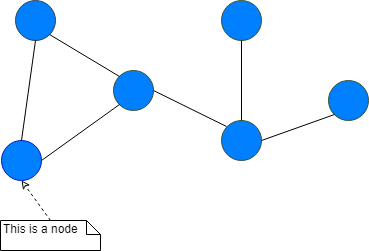
\includegraphics[width=4cm]{Figures/network}
\caption{Peer-to-peer network}
\end{figure}
\medskip

Each node has three responsibilities :

\begin{itemize}
  \item Keeping a copy of confirmed transactions, which is the blockchain itself.
  \item Validating a transaction if it's following the rules.
  \item Sharing information with their neighbors such as unconfirmed but valid transactions and mined blocks.
\end{itemize}

\clearpage

\begin{aside}

\paragraph{C ++ Code}

We've written a C++ code to simulate blockchains focusing on the mining process. The code is written in C++ using the library MPI to parallelize the process. Moreover, the executions were made on the Geneva University cluster to truly parallelize the code.

A full part is dedicated to the results we found in these simulations. \newline

Thus, we can simulate several miners trying to mine blocks and keep the blockchain synchronized. The goal is to deeply understand the network structure and to observe the evolution of the blockchain in the time. \newline

All along with the presentation of the blockchain's principles, we'll show the implementation in our code.

\end{aside}
\medskip

  \subsection{Transaction}

The main feature of the blockchain is to record transactions.

A transaction is composed of a list of inputs and a list of outputs (see Figure~\ref{transaction}). Outputs can include the payer itself. \newline

While doing a transaction, one wants to be sure that the payer is the true owner of the money. Then, to check this,  we use digital signatures :

\begin{itemize}
  \item The inputs of the transaction are encrypted with the public key of the payer.
  \item To prove he owns the coins, the payer "unlock" them by decrypting the signature with his private key.
  \item Then, he "locks" the outputs with the public key of the payees.
\end{itemize}

Technically, this is done with scripts linked to each input and output (see \cite{broken_crypto_primitives} for more details).


\begin{figure}[ht]
\centering
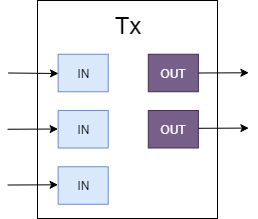
\includegraphics[width=4cm]{Figures/Transaction}
\hspace{1cm}
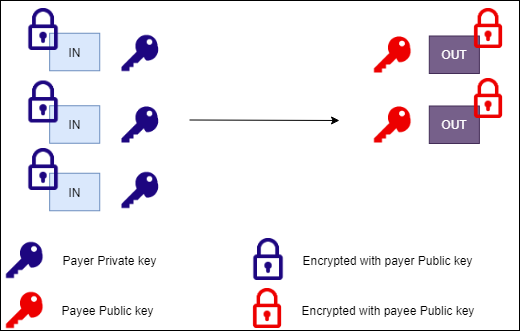
\includegraphics[width=8cm]{Figures/Transaction2}
\caption{A transaction diagram and digital signatures}
\label{transaction}
\end{figure}
\medskip

\begin{aside}

\paragraph{C++ code}

As we mentioned, the code focus on the mining process so we've simplified transaction management. \newline

In our simulation, a transaction is just a string, for example: (each line is a transaction) \newline

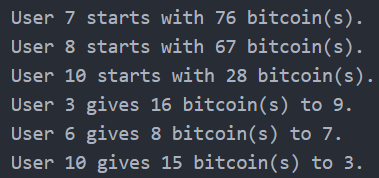
\includegraphics[width=6cm]{Figures/transactionsExample}
\medskip

So we don't have to manage signatures, inputs and outputs and it won't affect the mining process.

\clearpage

To generate those transactions, we've created a specific generator which creates a given number of transactions with limitations in the amount of money exchanged for a given number of users. \newline

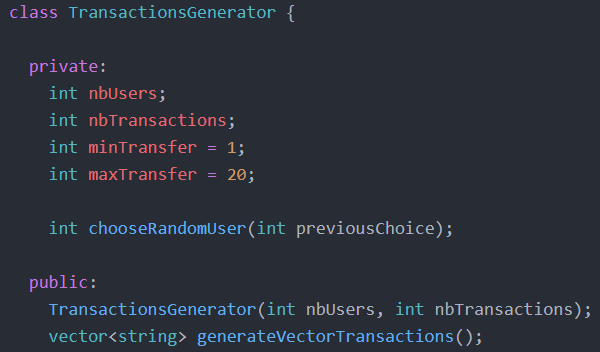
\includegraphics[width=10cm]{Figures/ClassTransactionsGenerator}
\medskip

\end{aside}
\medskip


  \subsection{Block}

Now that we have a transaction, we can transmit it to a node of the network. There, it needs to pass verification and if it's correct, it will be broadcast to other nodes. \newline

Once the transaction is accepted by a node, it will stay in a special area called the Mempool (Memory pool), this is where all unconfirmed transactions wait to be added in a block. A node can prioritize the transactions in its Mempool, especially if he's running out of memory, he can choose the order of arrival or, more probably, the highest transaction fee.

When a node receives the information that a new block has been added to the blockchain, he removes all newly confirmed transactions from his Mempool.  \newline

To form a new block candidate, a miner gathers transactions from the Mempool. Then, he will try to mine this block to add it to the blockchain. The miner will also add a block header which gives more information about the block (see \ref{blockHeader}). \newline

\begin{figure}[ht]
\centering
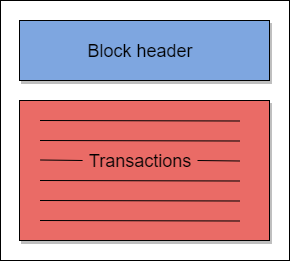
\includegraphics[width=4cm]{Figures/block}
\caption{A transaction diagram and digital signatures}
\end{figure}
\medskip

\begin{aside}

\paragraph{C++ code}

A block is an object with the following fields: \newline

\begin{itemize}
  \item A vector of string representing the transactions.
  \item A block header (see explanations below).
  \item An ID to get its position in the blockchain.
  \item We also add a reference to the previous block, this is used to build the blockchain.
\end{itemize}
\medskip

\clearpage
\medskip
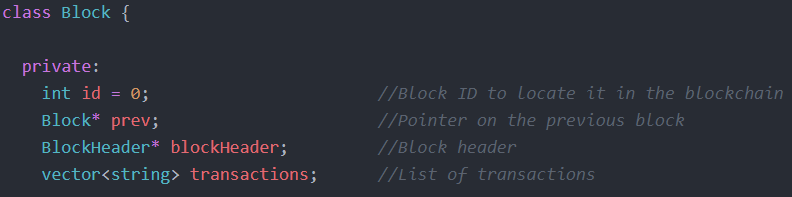
\includegraphics[width=10cm]{Figures/ClassBlock}
\medskip

A block can also build the Merkle tree with its transactions and be added in a blockchain.

\end{aside}
\medskip

  \subsection{Block header} \label{blockHeader}

A block header is a summary of the block, it's like its metadata. A block header contains six fields: \newline

\begin{tabular}{lll}
   version & The block's version & 4 bytes\\
   hashPrevBlock & The previous block's hash & 32 bytes \\
   hashMerkleRoot & The Merkle root representing all transactions in the block (see \ref{merkleRoot}) & 32 bytes \\
   time & The Unix time at which the block header was hashed & 4 bytes \\
   target & This is a shortened version of the target (see \ref{target}) & 4 bytes \\
   nonce & A random number  & 4 bytes \\
\end{tabular}

We'll see later that block headers are used for mining (see \ref{mining}).

\begin{aside}

\paragraph{C++ code}

As we've just seen, a block header contains all the fields mentioned: version, previous block hash, Merkle root, time, target and the nonce. \newline

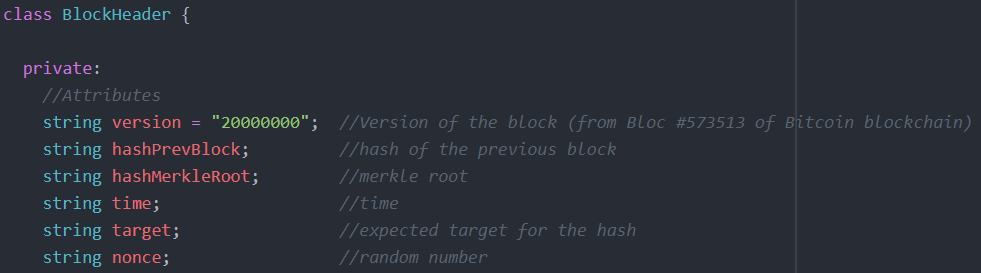
\includegraphics[width=14cm]{Figures/ClassBlockHeader}
\medskip

The version is always the same in our simulation because it won't affect mining. In the real world, the version helps to decode the block. A block header can set a nonce and compute its hash (by applying SHA256 twice).

\end{aside}
\medskip

  \subsection{Merkle root} \label{merkleRoot}

  As we've just seen, one of the block header fields is a Merkle root. Conceptually, it represents a fingerprint of the transactions' list and concretely it's just a hash.

  The blockchain uses Merkle trees for two reasons :

  \begin{itemize}
    \item To have a lightweight representation of the transactions because it results in only a hash.
    \item To be able to check if a transaction exists in a block without knowing all transactions in this block.
  \end{itemize}

  Merkle trees use a hash function, for blockchains, they use the same function than mining, which is

  SHA256(SHA256(.)).

  \begin{figure}[ht]
  \centering
  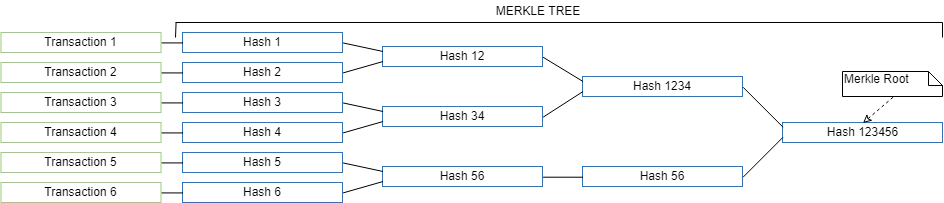
\includegraphics[width=\textwidth]{Figures/merkleTree}
  \caption{A Merkle tree}
  \end{figure}
  \medskip

  The main advantage of this technology is the speed and the ease to verify if a transaction belongs to a block. We don't need to know all transactions of the block and we don't even need to reveal any data from the transactions but only their hashes. \newline

  For example, if we want to check if the transaction 3 belongs to the block in our previous figure. We have to know its hash (Hash 3), Hash 4, Hash 12 and Hash 56. With those hashes, we can reconstruct the Merkle root. If it's the same, this means that the transaction 3 belongs to the block and that no transaction has been modified so the whole block is correct.


  \begin{aside}

  \paragraph{C++ code}

  We've created a class to build the Merkle tree from a vector of string and to return the Merkle root. \newline

  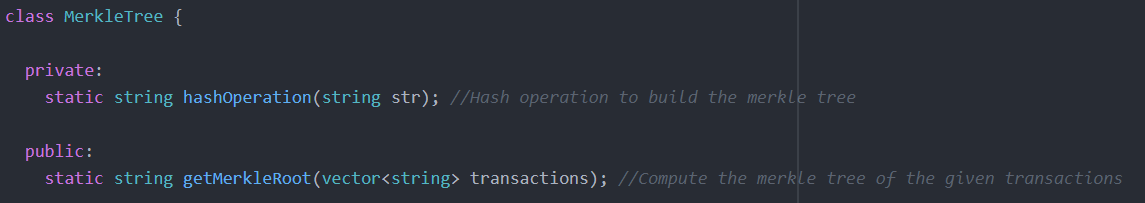
\includegraphics[width=14cm]{Figures/ClassMerkleTree}

  \end{aside}
  \medskip

  \subsection{The network}

  With all the concepts presented above, we can create a transaction, add it in a block, which will be mined thanks to its block header. Now, let's see how the nodes in the network secure the blockchain together. \newline

  The strength of the blockchain lies in its network because each node keeps a complete or partial copy of the blockchain. To keep the network updated, the nodes constantly share information between them. Typically, to broadcast a new transaction or a newly mined block :

  \begin{figure}[ht]
  \centering
  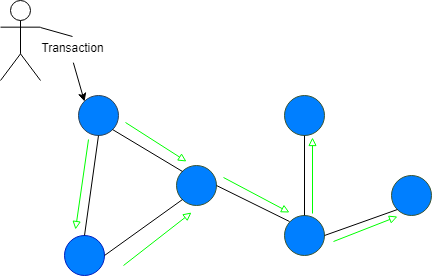
\includegraphics[width=5cm]{Figures/networkTransaction}
  \hspace{1cm}
  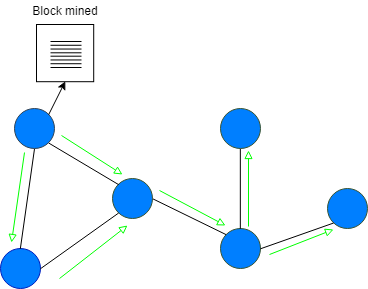
\includegraphics[width=5cm]{Figures/networkBlock}
  \caption{Communication inside the network}
  \end{figure}

  Then, each node updates its version of the blockchain. Now, one can wonder what happens if a node receives two different mined blocks at the same time?

  The node will fork the blockchain and have two versions of it and he will keep accepting blocks for both chains. As long as they have the same length, the node will choose to work on one of the chains but if one chain becomes longer, the node will keep it and forget the other one.

  \begin{figure}[ht]
  \centering
  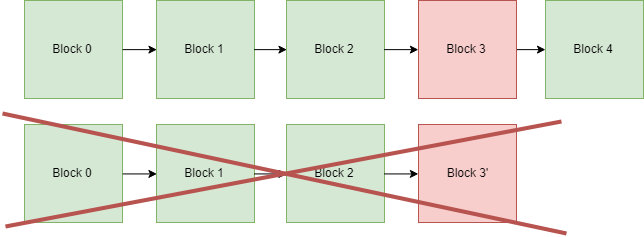
\includegraphics[width=5cm]{Figures/forkChains}
  \caption{Fork chains}
  \end{figure}

  The blockchain is always the longest chain created because it's the one that has requested more work of mining. This means that to have control over the blockchain, an attacker should have the majority of the computational power (at least 51\%). \newline

  \begin{aside}

  \paragraph{C++ code}

  As we said, the network is composed of miners so we implement mines as an object with the following fields: \newline

  \begin{itemize}
    \item An ID
    \item A vector of string to describe his mempool.
    \item A vector of blockchains to describe his versions of blockchains including forks.
  \end{itemize}
  \medskip

  \clearpage

  \medskip
  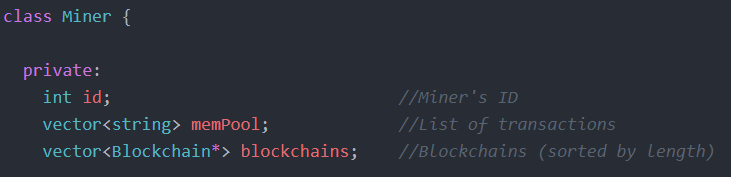
\includegraphics[width=10cm]{Figures/ClassMiner}
  \medskip

  A miner can fill a new block with transactions from his mempool, mine a block and add a block to one of his blockchains.

  Miners also have some functions to communicate through the network. For example, to serialize and deserialize blockchains (because only serializable objects can be sent in the network) or to handle a block the miner received. \newline

  Finally, blockchains are represented as linked lists with basic operations like adding a block or consult the last block. \newline

  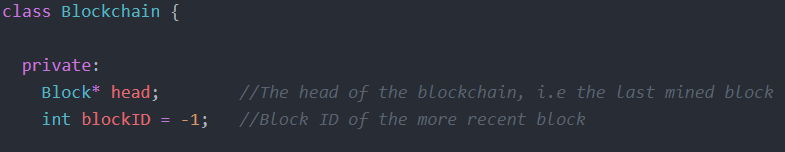
\includegraphics[width=10cm]{Figures/ClassBlockchain}

  \end{aside}
  \medskip

    \subsection{Bitcoin Block example}

  Bitcoin blockchain is public, we can follow the evolution on web sites like www.blockchain.com (\cite{blockchain_web_site}). We can see the fields we described and some other details, for example: \newline

  \begin{figure}[ht]
  \centering
  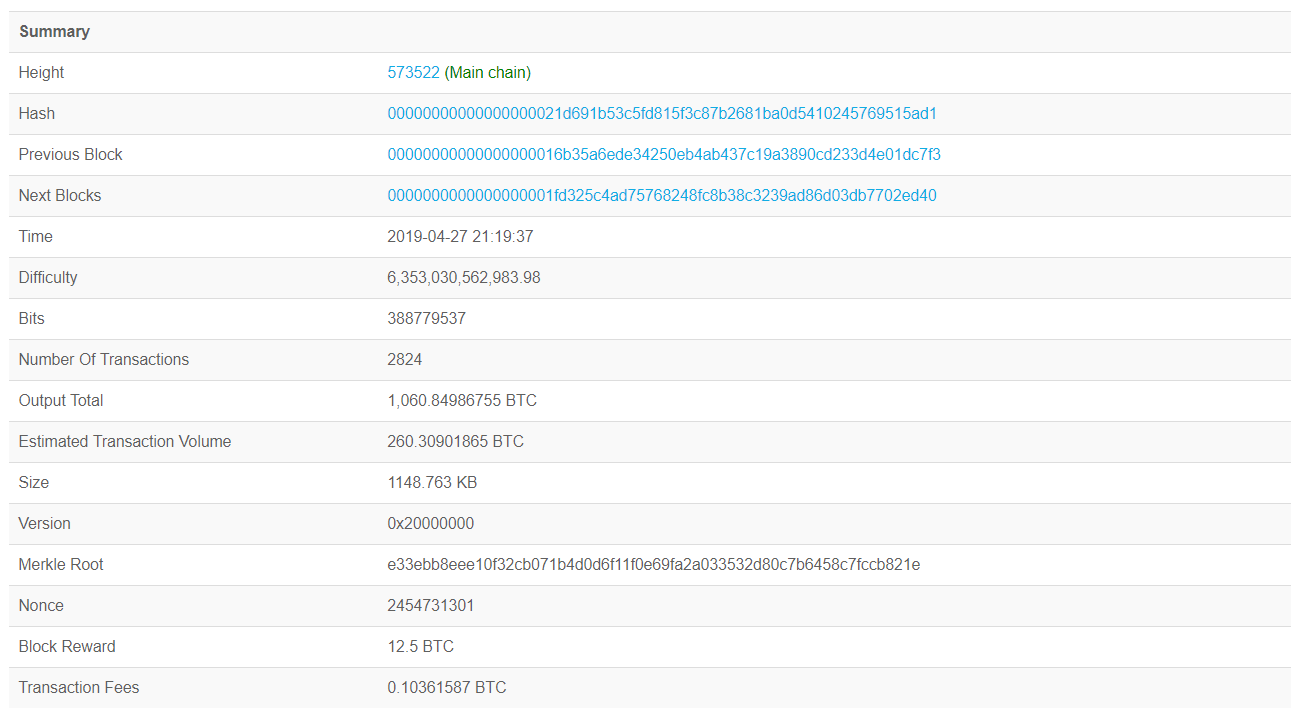
\includegraphics[width=15cm]{Figures/Block573522}
  \caption{Example of a Bitcoin block}
  \end{figure}

  \clearpage


  \section{Blockchain mining} \label{mining}

In this section, we give a general view of the mining process and the math involved.

  \subsection{Proof of work}

As we've seen before, blockchains lie on networks. Some nodes in these networks are miners, their role is to create a block of transactions and to mine it to add it to the network. \newline

How do they mine it? \newline

They hash the block header with a specific function : $H_M(x) = SHA256(SHA256(x))$.

This is an easy and fast operation for miners but they need to fulfill a condition: the resulting hash has to be under a target value.

  \paragraph{The target} \label{target}

In the block header, this target is described by a field, which is 4 bytes long.

Let's take an example: if the target field is: \newline

Target : 0x12\textcolor{orange}{07e540} \newline

12 is the exponent, it's a hexadecimal number and represents 18 in base 10. This means the target will be 18 bytes long.

\textcolor{orange}{07e540} is the coefficient. The exponent gives us a long series of zeros and we replace the 3 first bytes by the coefficient. \newline

This will give us : \textcolor{orange}{07e540}000000000000000000000000000000 . \newline

The miners have to find a hash lower than the target value. We can see this condition from another angle, the hash will be 256 bits (32 bytes) long but the target is shorter. So there is a difference of bits, let's note d, this means that the hash will have to start with at least d zeros to fit the condition. \newline

The target is not chosen randomly, it is set so a block will take about 10 minutes to be mined. This way, the number of blocks added in the network is controlled and allows enough time for the mined blocks to be broadcasted on the network.

The difficulty is updated about every two weeks, every 2016 blocks exactly. It depends on the expected time (2016 x 10 minutes) and the actual time.

  \paragraph{The nonce}

The last question remaining is how do miners affect the hash. They use another field of the block header, the nonce. This is the only field the miner can change, so the nonce is simply a random number and the miner's goal is to find the right random number which gives a hash lower than the target. \newline

This describes an algorithm called the proof-of-work.

  \paragraph{The rewards}

Then, we have a working protocol for mining but one can wonder why nodes will be willing to work for the blockchain.

It's quite simple actually, once a node has mined a block, he receives a reward (in Bitcoin if he works for Bitcoin blockchain). This is a way to motivate miners to work according to the rules for the blockchain. \newline

Miners have also another way of earning money, the payers may add a fee to their transaction. This transaction fee will be taken by the miner which confirms the transaction in a mined block.

As we've seen before, miners have a Mempool and they will prioritize the transactions according to the fees they can obtain. This is a way for payers to speed up transactions in the network which is often highly congested.


  \subsection{Hash functions}

In this work, we'll analyze the potential consequences if the hashing function for mining is broken. So let's recall some properties about hashing functions. \newline

The function used by mining is $H_M(x) = SHA256(SHA256(x))$.

Essentially, we can describe hash functions as deterministic functions, easy and fast to compute, whose output completely changes if the input changes and knowing the output gives no information at all on the input.

More precisely, hash functions, like SHA256, hold three properties: \newline

\begin{enumerate}
  \item Pre-image resistance: knowing $y_1$, it's difficult to find $x_1$ such that $h(x_1) = y_1$.
  \item Second pre-image resistance: knowing $x_1$, it's difficult to find $x_2$ such that $h(x_1) = h(x_2)$.
  \item Collision resistance: it's difficult to find pairs $(x_1, x_2)$ such that $h(x_1) = h(x_2)$.
\end{enumerate}


  \section{Uses in the world}

Now that we've understood the principles of blockchains, we may wonder who and what for people use blockchains nowadays.

\paragraph{Why people use blockchains instead of others security methods ?}

We can suggest a few reasons to answer this question (see \cite{blockchainPros}) :

\begin{itemize}
  \item Blockchains are fast, secure and transparent. Moreover, history has proven its robustness since no attacks were resulting from a weakness inside the blockchain itself.
  \item In general, people have a great opinion of it: 84\% think it's provided more security than others methods.
  \item There is around 70\% cost savings on business operation and 30 - 50 \% on compliance.
\end{itemize}

\paragraph{What for people use blockchains ?}

In the few last years, we've seen a lot of new blockchains being launched in different fields. We can have a look at some of them (see \cite{usesBlockchain})\newline

\begin{figure}[ht]
\centering
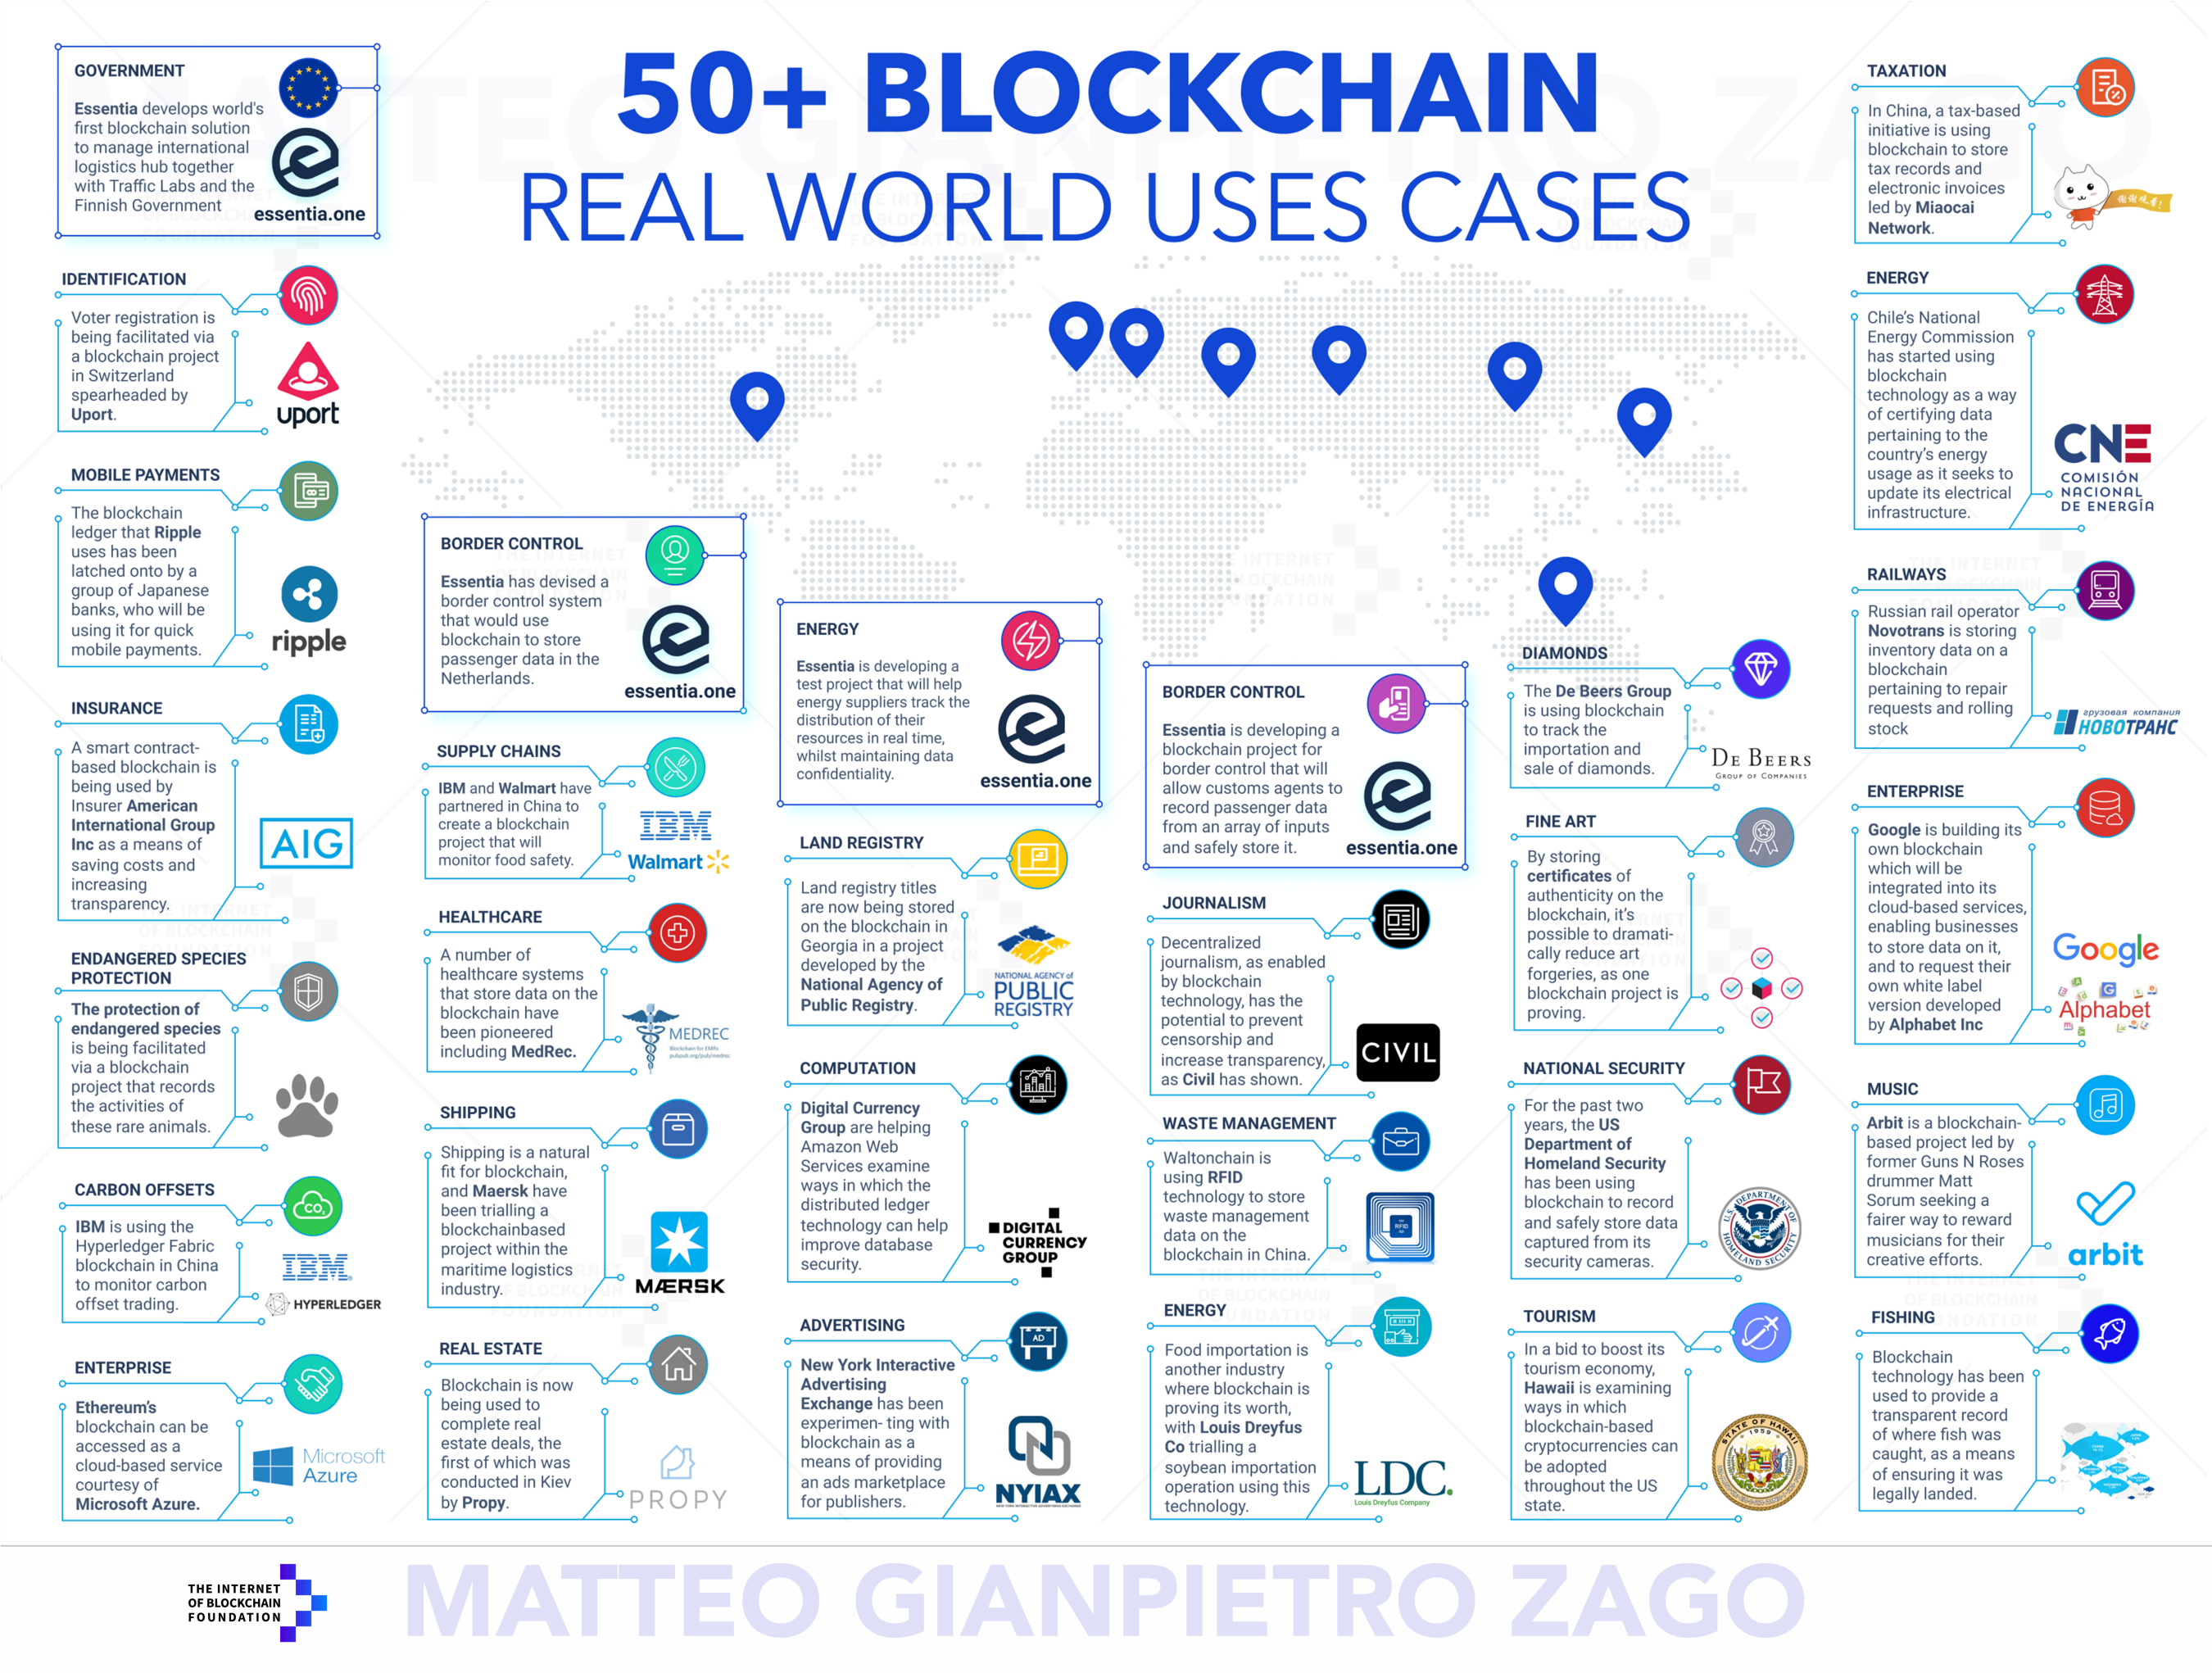
\includegraphics[width=10cm]{Figures/blockchainUses}
\caption{Blockchain uses in the world (see \href{https://medium.com/@matteozago/50-examples-of-how-blockchains-are-taking-over-the-world-4276bf488a4b}{Link to medium.com})}
\end{figure}
\medskip

We see that blockchains are used by governments for taxation and border controls, in the energy field and social field for insurance and healthcare for example.


\chapter{Blockchain simulation}

  As explained in the previous part, we've created classes to represent some features related to blockchains. Thus, we can instantiate miners, blocks, block headers and blockchains.

\section{Sequential code}

Then, the first version of the code is about making these objects to work together. This is a sequential version where, in the end, we have one miner able to create blocks, mine them and build his blockchain.

When the job is done, we display the state of the blockchain: \newline

\begin{figure}[ht]
\centering
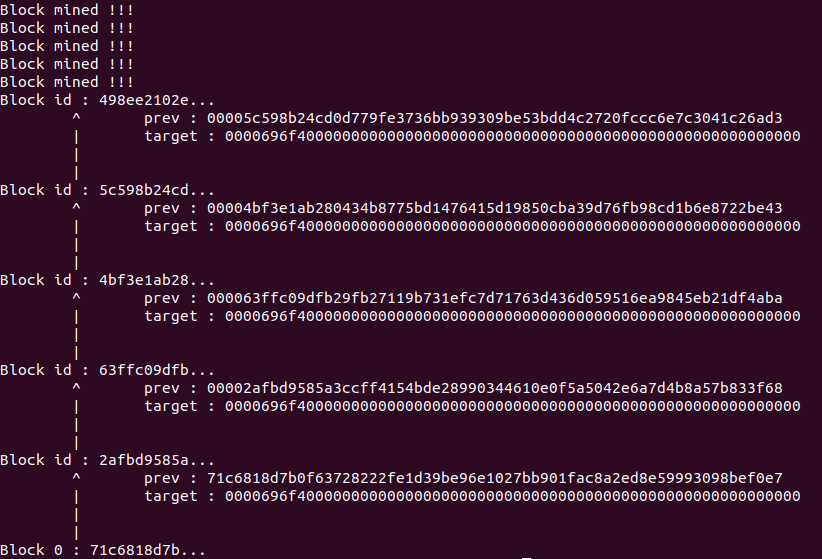
\includegraphics[width=10cm]{Figures/sequentialCode}
\caption{Example of execution}
\end{figure}
\medskip

We don't further in the analysis because the objective is to parallelize this code.

\section{Parallel code}

\paragraph{Transactions management}

As we mentioned, transaction management is simplified. So we decide to generate transactions with our specific generator and to communicate these transactions to all the miners. \newline

Thus, the first challenge is to generate and broadcast transactions. We arbitrary choose the miner 0 to generate the transactions, then he will serialize and broadcast them to the other miners.

At the same time, we manage the reception of these transactions by the others. They deserialize them and push them to their mempool. \newline

\paragraph{Communication through the network}

The more important challenge is to make the miners communicate about blocks they discovered. To do so, we created the following algorithm:

\clearpage

\begin{algorithm}
  \caption{Communication between miners}
  \begin{algorithmic}

    \WHILE{the mempool isn't empty}
      \STATE We fill a new block with transactions from the mempool

      \WHILE{No message received \&\& no block mined}
        \STATE We try to mine the block

        \IF{Block mined}
          \STATE We write related information into a log file
          \STATE We broadcast the block mined
        \ENDIF

        \STATE We check for messages

        \IF{Block received}
          \STATE Block reception algorithm (see below)
        \ELSIF{Blockchain received}
          \STATE We add the blockchain to ours
          \STATE We sort our chains to work on the longest
        \ELSIF{Blockchain request received}
          \STATE We send back the requested blockchain
        \ENDIF

      \ENDWHILE
    \ENDWHILE
  \end{algorithmic}
\end{algorithm}

\begin{algorithm}
  \caption{Block reception}

  \begin{algorithmic}
    \FOR{All our blockchains}
      \IF{The new block is the next one}
        \STATE We add it at the end
      \ELSIF{The new block is the last one}
        \STATE We do nothing
      \ELSE
        \FOR{All blocks in the chain}
          \IF{The new block and the current one are the same}
            \STATE We sent back this chain
          \ELSIF {The new block is the next of the current one}
            \STATE We create a forked chain including the new block
            \STATE We sort our chains
            \STATE We send our version of the chain
          \ENDIF
        \ENDFOR
      \ENDIF
    \ENDFOR

  \end{algorithmic}

\end{algorithm}

\subsection{Extra features}

\paragraph{Tests}

It's important to regularly test our code, especially to check if the communications are complete because this kind of error is quite hard to detect. There are some dedicated libraries to test our code but, in our case, we used a direct way by implementing functions to test our functions and print the results so we can check if everything is all right. \newline

We can test sending and receiving a block, a blockchain or an empty blockchain. This increases our confidence in the code robustness.

\paragraph{Frequency estimation}

We've seen that the computational power of a miner is important because the higher his computational power the faster he will mine. Then, we created a code to estimate the frequency of a miner. \newline

To estimate the frequency, we use the instruction RDTSC (ReaD Time Stamp Counter) which read the value of the register TSC. This register counts the number of cycles since the last reset. So we use the following algorithm to compute the number of cycles in 1 second: \newline

\begin{algorithm}
  \caption{Frequency estimation}

  \begin{algorithmic}
    \STATE int nbCycle = rdtsc()
    \STATE Wait for 1 second
    \STATE frequency = rdtsc() - nbCycle
  \end{algorithmic}
\end{algorithm}
\medskip

\paragraph{Logs}

All along the code, we write information in the log files to help analyze the blockchain at the end. For example: \newline

\begin{itemize}
  \item {[freq]} 2.4225  $\rightarrow$ Indicates the miner computational power in GHz.
  \item {[Tue Jul 23 17:40:48 2019]} 3fd2146979 26027 $\rightarrow$ Indicates the miner has mined a block with the exact time, the block ID and the duration in milliseconds.
  \item {[nbChains]} 1 $\rightarrow$ Indicates the number of forks chains the miner has made.
  \item {[i]} 47a9270fb6 $\rightarrow$ Indicates the beginning of the ith chain and its first block.
\end{itemize}
\medskip

\begin{figure}[ht]
\centering
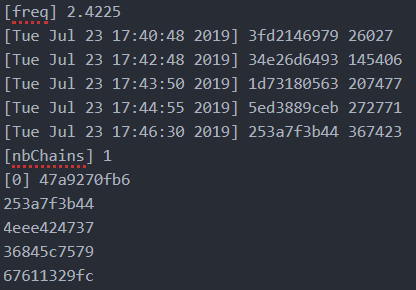
\includegraphics[width=8cm]{Figures/logExample}
\caption{Example of a log file}
\end{figure}
\medskip

We also write a general log file with the following data: \newline

\begin{itemize}
  \item {[nbTransactions]} 1000 $\rightarrow$ Indicates the number of transactions.
  \item {[nbProc]} 20 $\rightarrow$ Indicates the number of miners.
  \item {[difficulty]} 3 $\rightarrow$ Indicates the difficulty for the target (i.e. the number of zeros required at the beginning of the hash).
  \item {[finalTime]} 389194 $\rightarrow$ Indicates how long it took to complete the execution in milliseconds.
\end{itemize}



\section{Results}

\paragraph{Reading the logs}


\begin{enumerate}
  \item We read the file with the general data: nbProc, nbTransactions, difficulty.
  \item We read the file of each miner to get his frequency, the block mined and the blockchains.
  \item From the longest chain, we determine which miner has won a reward.
  \item We extract the data to display the timeline of the longest blockchain.
  \item We extract the times where the blocks were mined to compute statistics.
\end{enumerate}
\medskip

In the end, we display a table summing up the rewards and the forks of each miner, another table with statistics about the time needed to mine blocks and a timeline of the blockchain 10 blocks by 10 blocks. \newline

The following results were produced on the Geneva University cluster with a target starting with 5 zeros.

\paragraph{Analysis of the rewards and forks table}

This table is interesting in two points: \newline

\begin{enumerate}
  \item To analyze if the frequency and the number of rewards are correlated. In reality, the more a miner has computational power, the faster he should mine. \newline

  In our case, all miners have the same frequency because they were all located on the same node of the cluster.

  \item To observe the number of forks because this number is directly linked to the number of messages. If the number of forks is low, it means the consensus was obtained straight forward. On the other hand, if this number is high, it means the miners exchanged a lot of messages and probably wasted time on mining blocks which were finally not in the longest chain. \newline

  In our case, we see the number of forks is 1 for all miners so it means that our algorithm works well.
\end{enumerate}

\begin{figure}[ht]
\centering
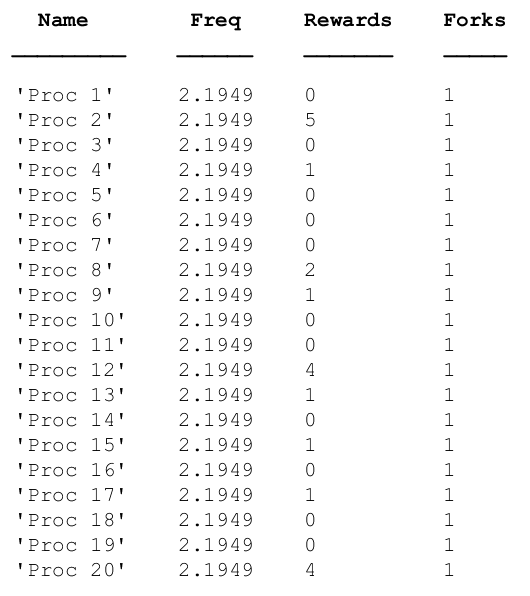
\includegraphics[width=10cm]{Figures/rewards}
\caption{Rewards won by the miners}
\end{figure}
\medskip

\paragraph{Analysis of the statistics table}

We can observe that the range is quite wide, from $\approx$ 9 minutes to 7 seconds, it means that some miners mined a block very quickly whereas some others took more time. This is because we choose the nonce in a uniform distribution so it's completely possible to obtain a right nonce after a few tries only. \newline

We can also note that the average time to mine a block is around 1 minute and 48 seconds, it's an arbitrary choice compared to the 10 minutes for the original blockchain.
\clearpage

\begin{figure}[ht]
\centering
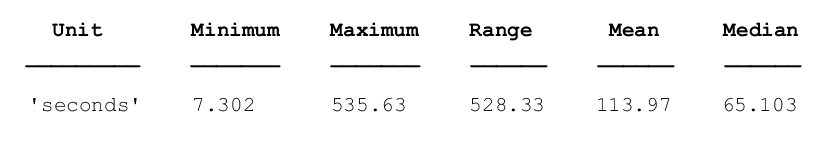
\includegraphics[width=10cm]{Figures/stats}
\caption{Statistics about the time needed to mine a block}
\end{figure}
\medskip



\paragraph{Analysis of the timeline}

When we study a new technical object, it's always interesting to look at its evolution in time. We choose the longest chain, in our case, there is only one fork so it's easy to choose. We display the blocks, 10 by 10, according to the time they were mined.

\begin{figure}[ht]
\centering
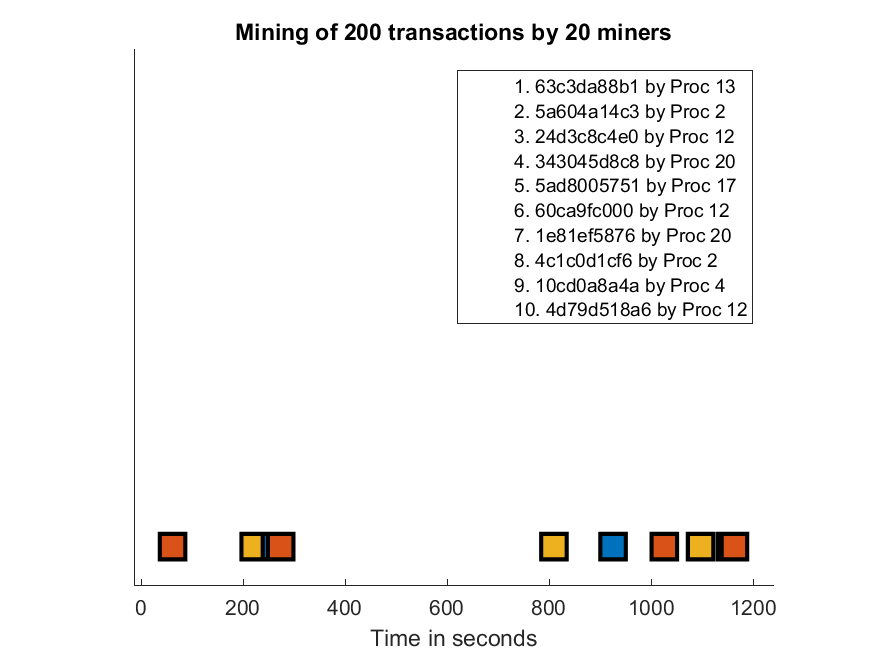
\includegraphics[width=10cm]{Figures/timeline_1}
\caption{Timeline for the 10 first blocks}
\end{figure}
\medskip


\section{Can we improve our model?} \label{improvements}

Here are some ideas to improve our simulation: \newline

\begin{itemize}
  \item The possibility to choose the network structure. To do so, we could use an adjacency matrix: \newline

  \begin{figure}[ht]
  \centering
  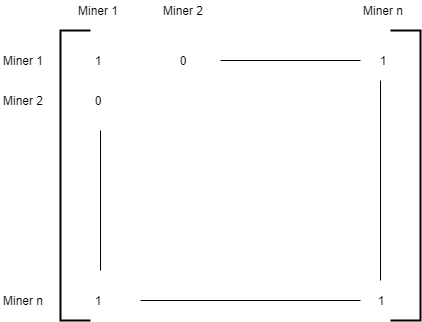
\includegraphics[width=8cm]{Figures/matrix}
  \caption{Example of an adjacency matrix}
  \end{figure}
  \medskip

  An adjacency matrix is symmetrical and 1 in the position (i, j) indicates that the miner i and j are neighbors. For example, in the figure above, the miner 1 and n are neighbors but not the miner 1 and 2. \newline

  With this method, we could try several network structures and analyze their influence on the mining process.

  \item The possibility to create pools. We could create a function which defines if a miner belongs in a pool or not: \newline

  \[
    isInPool(miner) =
    \begin{cases}
      0, & \text{if the miner doesn't belong in a pool}  \\
      i > 0, & \text{if the miner belongs to the pool i} \\
    \end{cases}
  \]
  \medskip

  Then, when a miner successfully mined a block, we share the reward with the pool if he belongs to one. With the method, we could try to implement the 51\% attack.

  \item Implementing the selfish mining attack. We've implemented the finite state machine which models this attack but we could also try to implement this algorithm for real to observe the results match.


\end{itemize}


\chapter{Breaking mining if SHA256 is broken}

	We know that mining is based on SHA256 so, in this part, we'll see different techniques (inspired from \cite{broken_crypto_primitives}) to win against traditional mining if SHA256 is broken.

\section{Pre-image with fixed Merkle root}

First, we analyze the probability for an attacker with a pre-image oracle to break mining, i.e. to get an high probability to solve the PoW before the other nodes in the network.

If we suppose we can have a pre-image oracle for SHA256, then we will be able to build an oracle for $H_M(x) = SHA256(SHA256(x))$ by applying the first oracle twice.

	\subsection{Input set of $H_M$}

As explained before, a miner applies the hashing operation $H_M(x)$ to the block header. A classic miner only controls the value of the nonce but an attacker will try to control more. \newline

The version, the previous block's hash and the merkle root are fixed fields. \newline

For the time field, the system allow a range of 7200 seconds around the current time. So, over the 32 bits dedicated for this field, an attacker will be able to control about 13 bits.

For the target, the protocol will check if the target value is at most the one defined by the consensus of the network, this means the attacker can control about 28 bits.

For the nonce, like any miner, the attacker can control the 32 bits allowed to it. \newline

The block header's size is $4 + 32 + 32 + 4 + 4 + 4 = 80$ bytes $ = 640$ bits.

An attacker can control $b = 13 + 28 + 32 = 73$ bits on the input value, which means he has $2^b$ possibilities to call the hash function $H_M$.

	\subsection{Output set of $H_M$}

The result of $H_M$ is an hash from SHA256, so it has a length of $n = 256$ bits and there are $2^n$ possibilities of outputs. \newline

Then, we've seen that to fulfill the condition given by the target, the hash needs to start with a specific number of zeros, let's note d zeros.

In reality, matching with the coefficient may require more effort (see \ref{appendixTarget} for more details). \newline

This means that there are $2^{n-d}$ hashes lower than the target.

	\subsection{Probability of breaking mining}


By calling $H_M$, one has a probability of $\frac{2^{n-d}}{2^n}$ to get a valid hash.

That way, we can get the number of correct pre-images i.e in the input set, how many inputs will end as a correct hash.

\begin{equation}
proba\_of\_correct\_hash \times \#possible\_inputs = \frac{2^{n-d}}{2^n} \times 2^b = 2^{b-d}
\end{equation}
\newline

\begin{figure}[ht]
\centering
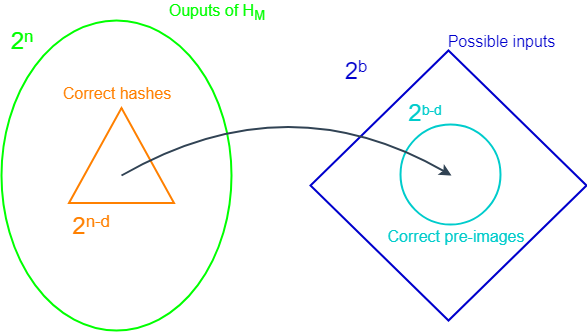
\includegraphics[width=8cm]{Figures/probaSuccess}
\caption{Probability of getting a correct pre-image}
\end{figure}
\medskip

In his attack attempt, the attacker queries the pre-image oracle for specific target hashes. So he will choose a correct hash (triangle set) and hope that the output is one of the correct pre-images. This is the probability that he gets an accepted pre-image.

\begin{equation}
\frac{\#pre-images}{\#accepted\_outputs} = \frac{2^{b-d}}{2^{n-d}} = 2^{b-n}
\end{equation}
\newline

Then, to get the real probability of success, we need to add a constraint on the number of queries allowed to the attacker. Because, otherwise, the attack won't be faster than the traditionnal mining. So let's consider the attacker can query the oracle $2^a$ times.

\begin{equation}
P_{success} = 2^a \times 2^{b-n} = 2^{a + b - n}
\end{equation}
\newline

Finally, we can estimate this probability of success. Let's take $a = 80$ so the attacker have $2^{80}$ tries (above this value, he may need more than 10 minutes to complete his attack). So, we have $P_{success} = 2^{80+73-256} = 2^{-103} \approx 10^{-32}$, which completely negligible.

Then, we can conclude that having a simple pre-image oracle doesn't help to break mining.


  \section{Pre-image with variable Merkle root}

  \subsection{Random Merkle root}

In the previous section, we've assumed that the Merkle root is a fixed field because we've supposed that the list of transactions was also fixed. \newline

But an adversary could try to work backward, to choose a random Merkle root and to try to reconstruct the Merkle tree leading to semantically valid transactions. By contrast with the previous method, the transactions are created by the attacker himself. However, even without figuring out any probabilities, we can conclude that this method is infeasible. That's because the reconstructed transactions will have to contain valid outputs and valid signatures.

  \subsection{Coin base transactions}

However, there is an exception for the previous remark based on two observations. First, the system doesn't have a constraint about the number of transactions in a block and second, each block has a coinbase transaction, which creates money as a reward for the miner. \newline

An attacker could create a block with only a coinbase transaction. These transactions have a fixed prefix and suffix and they have a length-variable field up to 100 bytes, scriptSig.

Then, the attacker can create a valid block by finding a valid Merkle root: $h(a || x || b) = T$, where x is the Merkle root, T is the target and a and b are the prefix and suffix of the block header.

Finally, he'll have to solve: $h(b || y || d) = x$, where y is the scriptSig and b and d are the prefix and suffix of the coinbase transaction. So the Merkle root match with a valid transaction.

($|| . ||$ means concatenation)\newline

Both predictions will have a pre-image with high probability but if not, the attacker can try with another target or with different lengths for the scriptSig. Nevertheless, his probability of success is very high.


  \section{Bounded pre-image oracle}


  \subsection{Construction of the oracle}

In reality, a hash function breakage can imply more powerful tools than a simple pre-image oracle. To cover this possibility, we can construct a general oracle (see \cite{broken_crypto_primitives}). \newline

This oracle takes as input : $(a, b, y_l, y_i, i, s) = (prefix, suffix, target\_low, target\_high, position, length)$. It will return $x_i$ such that : $y_l <= h(a || x_i || b) <= y_h$ or none (if there is no pre-image). \newline

In other words, the prefix, suffix and length of the pre-image are fixed, this allows us to have control over the format of the pre-image and, in our context, to fix some fields of the block header. The value will be between a target range, this will help us satisfy the condition given by the target.

The position of the pre-image is also specified, this means the same $x_i$ is returned on each call and a call on j will return $x_j \neq x_i$. \newline

Technically, the suffix is added to keep a symmetry but it's not needed for our attack. Moreover, in reality, this is usually the hardest part of the oracle to setup.

  \subsection{Attacks against mining}


An attacker with access to our bounded oracle can simply call for $(headerBeginning, none, 0^{256}, target, 0, 32)$. \newline

For recall, the target is 256 bits long, the block header is 32 bits and the headerBeginning is the beginning of the block header until the nonce. This will return a pre-image of 32 bits with the first fields of the block header and a correct nonce such that the hash is under the target value. \newline

This kind of attack will completely break mining, which allows the attacker to create deep forks and then, reverse transactions or double-spend.


  \section{Second pre-image and collision}

We've seen in the previous section vulnerabilities linked to pre-images. Let's have a look at second pre-images and collisions.

  \subsection{Attacks on blocks}

    \paragraph{Second pre-image}

Let's recall the theory about second pre-images: for a specific hash given by a specific input, a second pre-image oracle allow us to find another input giving the same hash.

In our context, one could want to replace a block by a new block with the same hash to maintain the blockchain valid, this way one could completely modify the blockchain.

However, this is concretely infeasible because more than just the hash, the new block has to be valid in terms of transactions. This means the transactions have correct inputs and correct signatures, the probability that the new block respects these constraints is almost zero. \newline

    \paragraph{Collision}

For collisions, the idea would be to create several blocks with the same hash and to insert them in the network. This would allow an attacker to be able to fork the chain and possibly double-spend or steal coins.
However, following the same remark we did for second pre-images, the probability to create valid blocks is negligible. \newline

To conclude, collisions and second pre-images are irrelevant to break mining.

  \subsection{Merkle roots}

As recall the hash function $H_M$ is also in Merkle trees, then one could alter already mined blocks by changing transactions but with the same Merkle root.

    \paragraph{Blocks inside the blockchain}

This idea would be to change the transactions in a block by getting a Merkle root with the same hash. As we expose before, the probability of getting valid transactions is very low. So the nodes will reject the modified block.

    \paragraph{New added blocks}

However, the situation is different if the adversary focuses on the last block. The attacker can create a new block with different transactions but the same Merkle root. Even if, this newly created block is invalid, the attacker can send it to the network and this may cause the nodes to reject both blocks or even to accept the invalid block.

This attack was done in July 2015 (\cite{mining_attack}), nodes were accepting invalid blocks and then, validating wrong transactions. Nowadays, a new version of the protocol has been released and these problems are solved. \newline

The adversary can also double-spend coins by creating a new block with conflicting transactions according to the valid block using a collision or second pre-image oracle. Then, he can transmit both blocks in the network, this will fork the blockchain and may fool the vendor.


  \section{Conclusion}

  \subsection{Consequences summary}

We can sum up the different consequences of breakages on SHA256. \newline

\begin{tabular}{ll}

  \underline{\textbf{Breakage}} & \underline{\textbf{Consequences}} \\
  Pre-image & Complete breakage of the blockchain \\
  Bounded pre-image & Complete breakage of the blockchain \\
  Second pre-image & Double spending, steal coins \\
  Collision & Double spending, steal coins \\

\end{tabular}

  \subsection{Contingency plans}

All the attacks presented above are based on potential SHA256 vulnerabilities. We cannot guarantee that SHA256 will stay safe forever. However, we can notice it was created in 2001 and no significant weaknesses have been discovered yet so we can conclude SHA256 is quite robust (see a StackExchange conversation about SHA256 security, \cite{SHA256_security}). \newline

In case SHA256 is broken, Bitcoin has a contingency plan (see \cite{contingency}).

As we've seen this situation would be dramatic, an attacker could compromise the whole system, this includes the alert system.

The plan in this situation is to ask the users to shut down their clients and to hardcode the public keys of all addresses that have unspent outputs. Then, these keys will be used when a new version of the blockchain is released. \newline

The code for all of this should be prepared but, in reality, this is not the case because, even if the consequences would be severe, the risk is very low.


\chapter{Attacks using mining weaknesses}

   In the previous chapter, we've seen that mining is based on SHA256 and we've analyzed the consequences if SHA256 is broken. In this chapter, we'll try to find some weaknesses in mining and use them to fool the process.

\section{Double-spending}

One of the very famous technic to trick a seller is called double-spending. As explained in \cite{double_spending_def}, a double-spending attack is used by a buyer to foul the seller, following the next steps :

\begin{enumerate}
  \item The buyer A broadcasts a transaction AB in the network where he pays seller B.
  \item The buyer A creates another block with a transaction $\overline{AB}$ which invalidates transaction AB.
  \item The buyer A secretly mines a branch on this new block.
  \item The buyer A waits that seller B sends his product.
  \item Once the buyer's branch is long enough, he broadcasts it which will deny transaction AB.
\end{enumerate}

With this method, the attacker uses his bitcoin twice, that's why it's called double-spending. \newline

\begin{figure}[h]
\centering
\captionsetup{justification=centering}
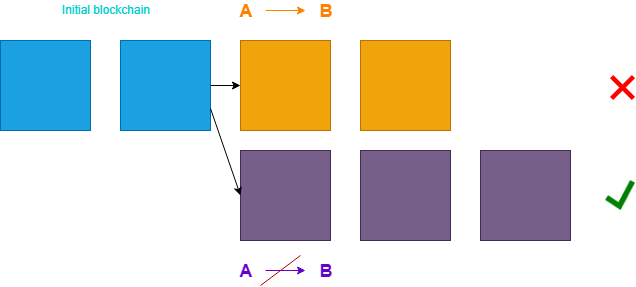
\includegraphics[width=8cm]{Figures/doubleSpending}
\caption{Double-spending - The longest chain will the purple one which invalidates the bitcoins sent to B while the seller has already sent his product}
\end{figure}
\medskip

\section{51\% attack}

  \subsection{What is it?}

The main difficulty to achieve this attack is to be able to build a longer chain to invalidate the transaction which gives bitcoins to the seller. One possible solution is the 51\% attack.

The 51\% attack has always been an important concern about blockchains' security. The main idea is that an attacker will control the majority of the computational power, i.e. at least 51\%.

\clearpage

\begin{pquotation}{Bitcoin glossary \cite{51Percent_definition}}
The ability of someone controlling a majority of the network hash rate to revise transaction history and prevent new transactions from confirming.
\end{pquotation}

In other words, an adversary with at least 51\% of the network will be able :

\begin{itemize}
  \item To prevent some users to do transactions, by systematically denying their transactions. Because the attacker controls the majority of the network, even if some nodes confirm the user's transaction, it will never be part of the longest chain.
  \item To reverse his transactions, this is double-spending.
\end{itemize}

  \subsection{Is it possible to implement it?}

    \paragraph{For Bitcoin}

To set a 51\% attack up, an attacker needs to gather enough mining computers to get more than 50\% of the computational power of the actual network.

Moreover, the attacker will have to supply enough electrical power to run those computers. \newline

Now, the real question is how much will it cost. We can try to estimate the cost for Bitcoin (see \cite{cost_bitcoin_51_attack}). \newline

First, buying specialized computers for mining will cost about \$2.4 million and \$250 million in infrastructure to install these computers and the equipment needed (like ventilation). \newline

Then, to power this structure, one will need around 30 Terawatts of electricity per year. For example, Morocco consumed 29 Terawatts in 2017 and Switzerland consumed 63 Terawatts the same year. All this electricity will cost around \$2 million by day. \newline

To sum up, a 51\% attack against Bitcoin will cost \$1.4 billion. This makes the attack almost impossible due to this huge cost, even for a large state-sponsored organization, it will be very complicated to set up this attack.

    \paragraph{What about other blockchains?}


We've studied the feasibility of Bitcoin which is one of the most famous blockchains nowadays and its network is now very large. But one can wonder if the threat is more important with smaller blockchains. \newline

Indeed, the cost for a 51\% attack decreases for smaller coins. However, for every serious blockchain, there are still thousands or millions of nodes and anyways, it would more profitable to mine honestly and win coins through rewards.

On \href{https://www.crypto51.app/}{Crypto51}, we can observe the cost to make a 51\% attack on different cryptocurrencies. \newline

\begin{figure}[h]
\centering
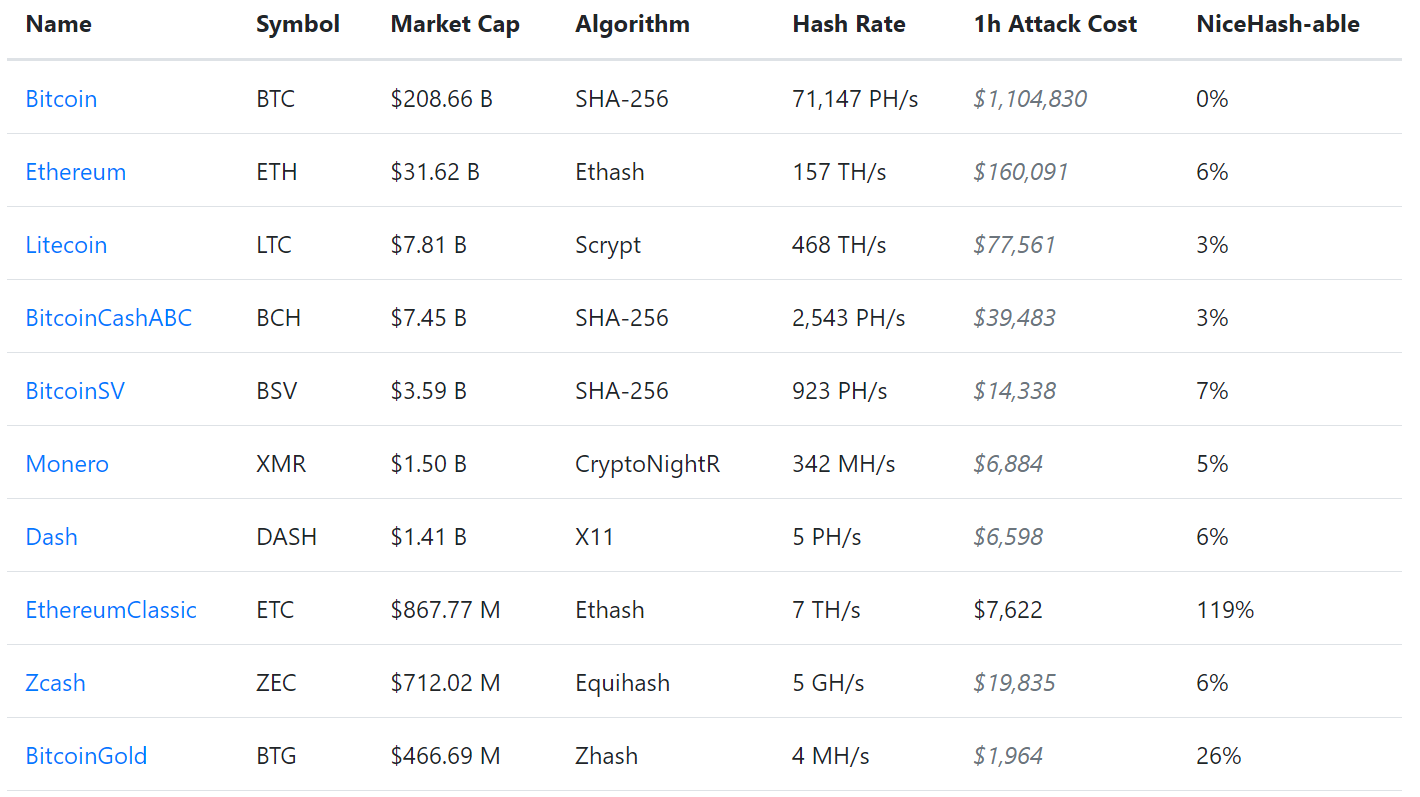
\includegraphics[width=8cm]{Figures/crypto51}
\caption{Crypto51}
\end{figure}
\medskip


Then, the probability remains low especially for the biggest blockchains. However, it can still happen (see \cite{blockchains_51_attack}). For example, EthereumClassic was attacked in January 2019 and it lost almost \$1.1 million in one day.

Preventing this attack can be very complicated but there are still some ideas :

\begin{itemize}
  \item Merging mining. Smaller cryptocurrencies can use mining power of larger ones so they become less vulnerable.
  \item Penalizing delayed blocks. The attacker mines blocks secretly and broadcasts them lately, a penalty will reduce the benefit of the attack.
  \item A detection algorithm for the 49\% left. Once the attack is detected, the 49\% left can try to acquire more power to stop the attack.
\end{itemize}


  \section{Selfish mining}

In the previous section, we've considered an attack to trick vendors by taking advantage of the system. Now, we will study a method to trick the system itself.

As we mentioned before, a node wins a reward when he successfully mines a block and adds it in the blockchain, the node earns the rewards as long as his block is in the blockchain. \newline

We will present the method of selfish mining, where miners try to increase their rewards allowed for mining (see \cite{majority_not_enough}).

  \subsection{What is it?}

First, let's suppose that all the computational power is divided into two groups: the first group follows the selfish mining strategy and the second group follow the classic mining strategy. \newline

The main idea of selfish mining is to mine secretly blocks in advance so the miners create a longer chain than the others. Then, at the right time, they reveal their chain which will become the new longest chain, so they win the rewards and waste the work of the other miners. \newline

Let's see in details how this strategy works, there are four important cases: \newline

\begin{itemize}
  \item Case 1: The honest miners find a new block on the public chain, the selfish miners will just adopt the new chain.
  \item Case 2: The selfish miners find a new block on the public chain, they will keep this block secret and then, there are two possibilities (Case 3 or 4).
  \item Case 3: The selfish miners have secretly one block in advance but the honest miners find a new block first and broadcast it, in that case, the selfish miners broadcast their secret block immediately. Since two blocks are broadcast almost at the same time, miners will have to choose which block they mine after. All the selfish miners will mine after their block, and the honest miners will mine on the first they receive. Let's note $\gamma$ the proportion of honest miners who mine after the selfish miners' block.
  \item Case 4: The selfish miners have secretly one block in advance and they find a new one, so they keep this new block secret. Then, they will try to keep two blocks or more in advance the longest time possible. If they only have one block left, they publish their secret chain.
\end{itemize}
\medskip

\begin{figure}[ht]
\centering

\subfloat[Case 1]{
  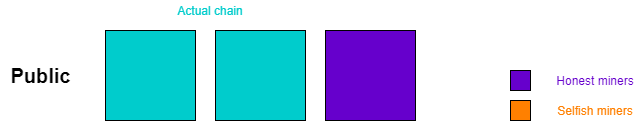
\includegraphics[width=6cm]{Figures/SM_1Honest}
}
\hspace{1cm}
\subfloat[Case 2]{
  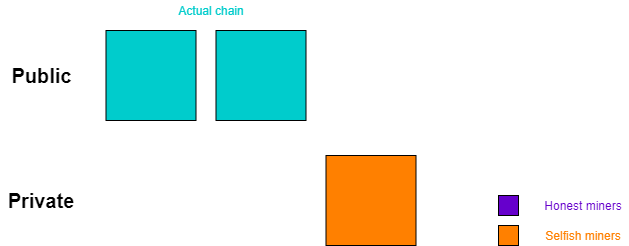
\includegraphics[width=6cm]{Figures/SM_1Selfish}
}
\end{figure}
\medskip

\begin{figure}[ht]
\centering

\subfloat[Case 3]{
  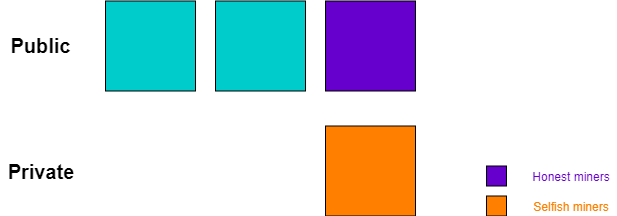
\includegraphics[width=6cm]{Figures/SM_2Honest}
}
\hspace{1cm}
\subfloat[Case 4]{
  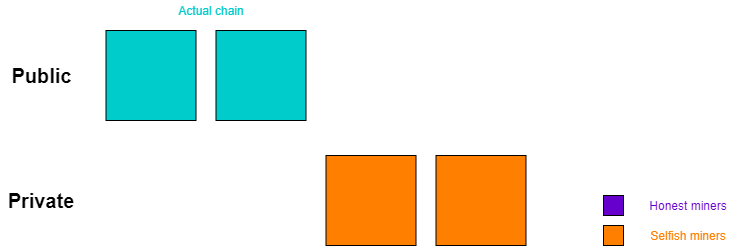
\includegraphics[width=6cm]{Figures/SM_2Selfish}
}
\end{figure}

  \subsection{Is it feasible?}

As we've just seen, this strategy is based on the fact that the selfish miners succeed in mining blocks ahead of the honest miners. To do so, it's obvious that their combined computational power will affect their chance of success, let's note $\alpha$ the computational power of the selfish miners.

As described in \cite{majority_not_enough}, we can represent the selfish mining algorithm with a finite state machine. \newline

\begin{figure}[ht]
\centering
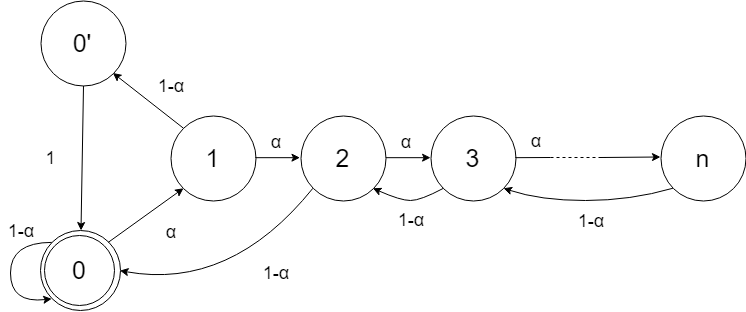
\includegraphics[width=10cm]{Figures/finiteState}
\caption{Selfish mining finite state machine}
\end{figure}
\medskip

In this machine, the initial state is the state 0 and it corresponds to case 1. The state 1 corresponds to case 2, the state 0' to case 3 and the states 2 and more correspond to case 4. \newline

We can compute the probabilities of this state machine, we note $p_i$ the probability of being in state i. From these probabilities, we can compute the rewards the selfish and honest miners will win. \newline

We can find more explanations about the formulas in this appendix \ref{appendixRevenue}. \newline

\begin{table}[ht]
  \centering

  \begin{tabular}{c}
    $r\_honest =  p_0 . (1 - \alpha) . 1 + p_{0'} . \gamma . (1 - \alpha) . 1 + p_{0'} . (1 - \gamma) (1 - \alpha) . 2$ \\
    \\
    $r\_selfish =  p_{0'} . \gamma . (1 - \alpha) . 1 + p_{0'} . \alpha . 2 + p_2 . (1 - \alpha) . 2 + P[i > 2] . (1 - \alpha) . 1$
  \end{tabular}
  \caption{Revenue won by the honest and selfish miners according to $\alpha$ and $\gamma$}
  \label{revenueFormulas}
\end{table}
\medskip

We can implement this finite state machine and try some values of $\alpha$ and $\gamma$.

\begin{figure}[ht]
\centering
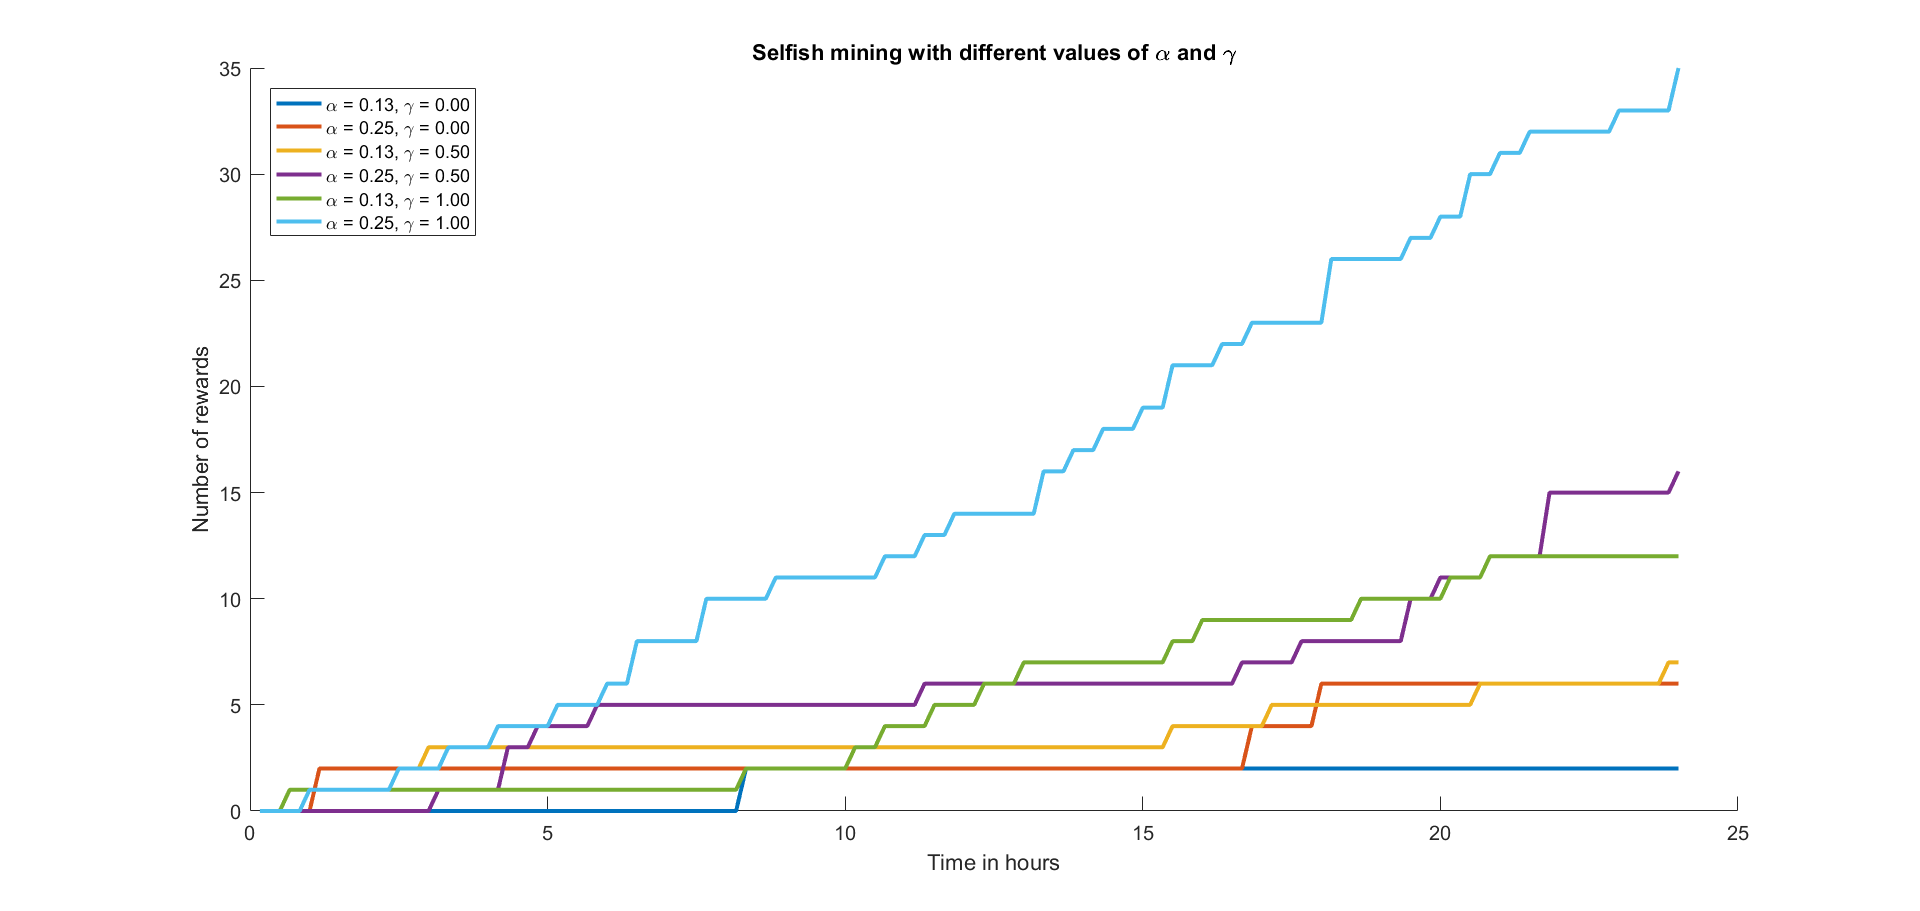
\includegraphics[width=12cm]{Figures/selfishGraph}
\caption{Rewards according to different $\alpha$ and $\gamma$}
\end{figure}
\medskip

We see that $\gamma$ and $\alpha$ are linked because the more $\gamma$ increases the more the pool size $\alpha$ needs to increase to win the same reward. Let's try several values of $\gamma$ with the hash rates of the four largest pools in Bitcoin network (see \cite{hashrate_pools}).

\begin{figure}[ht]
\centering

\subfloat{
  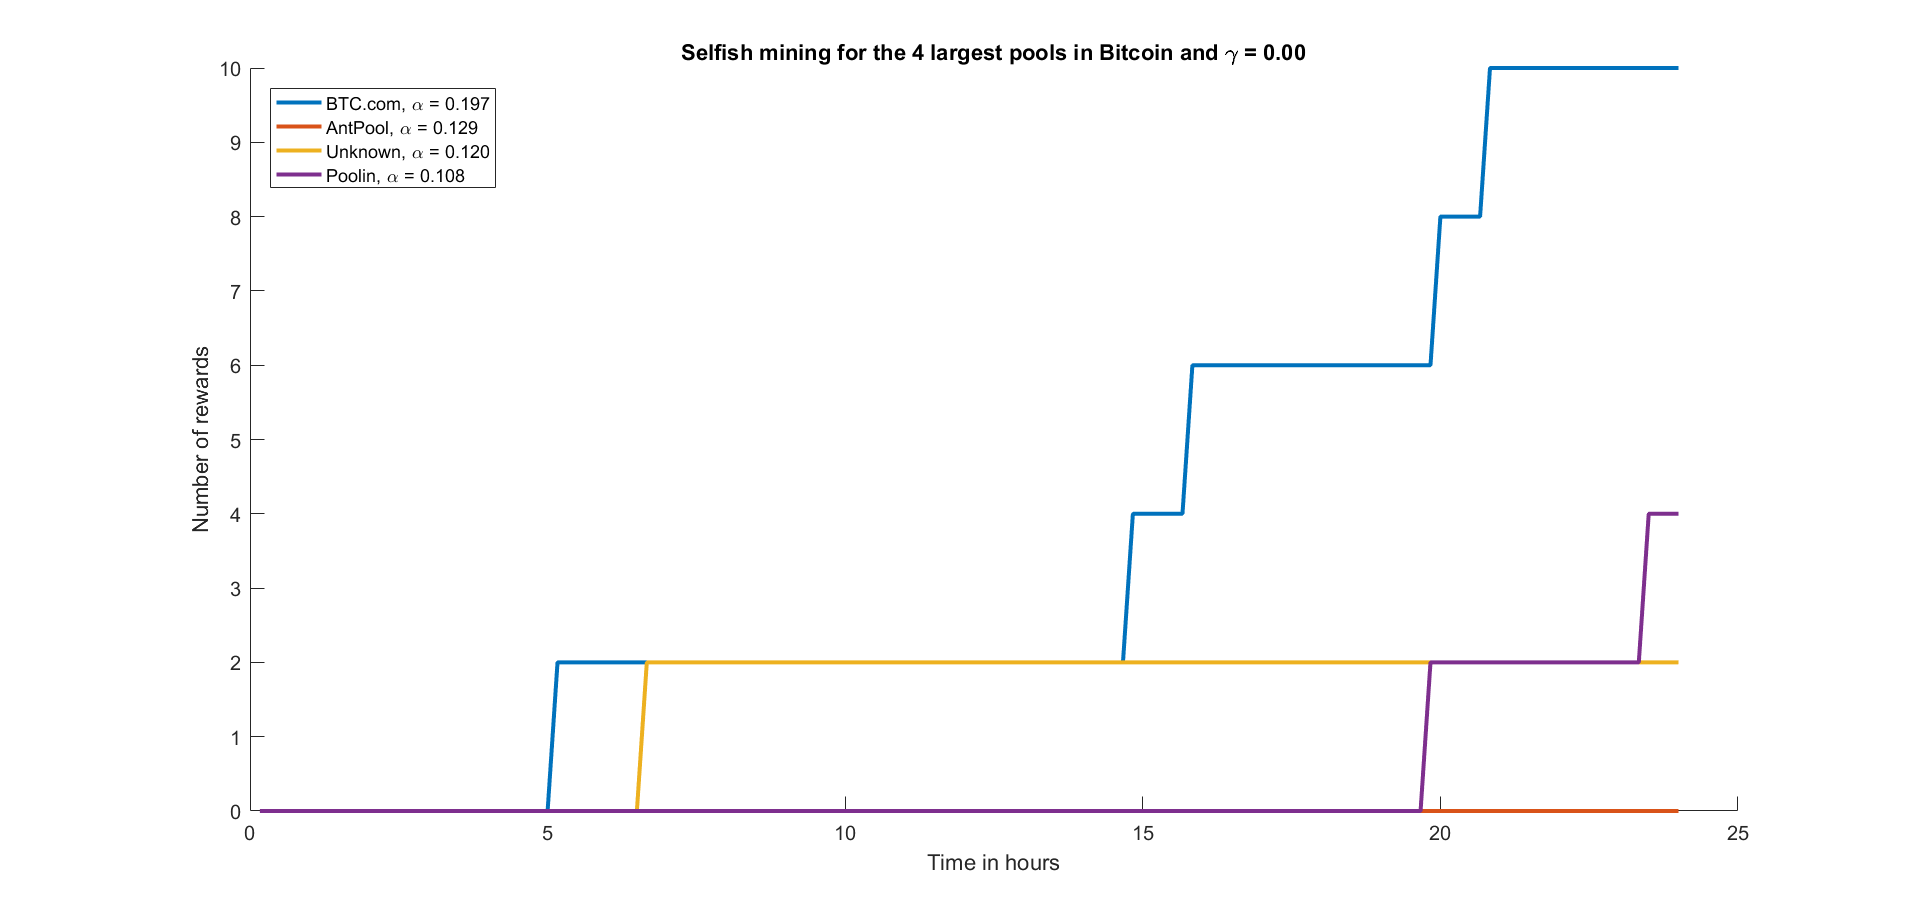
\includegraphics[width=12cm]{Figures/largestPools0}
} \newline

\vspace{1cm}

\subfloat{
  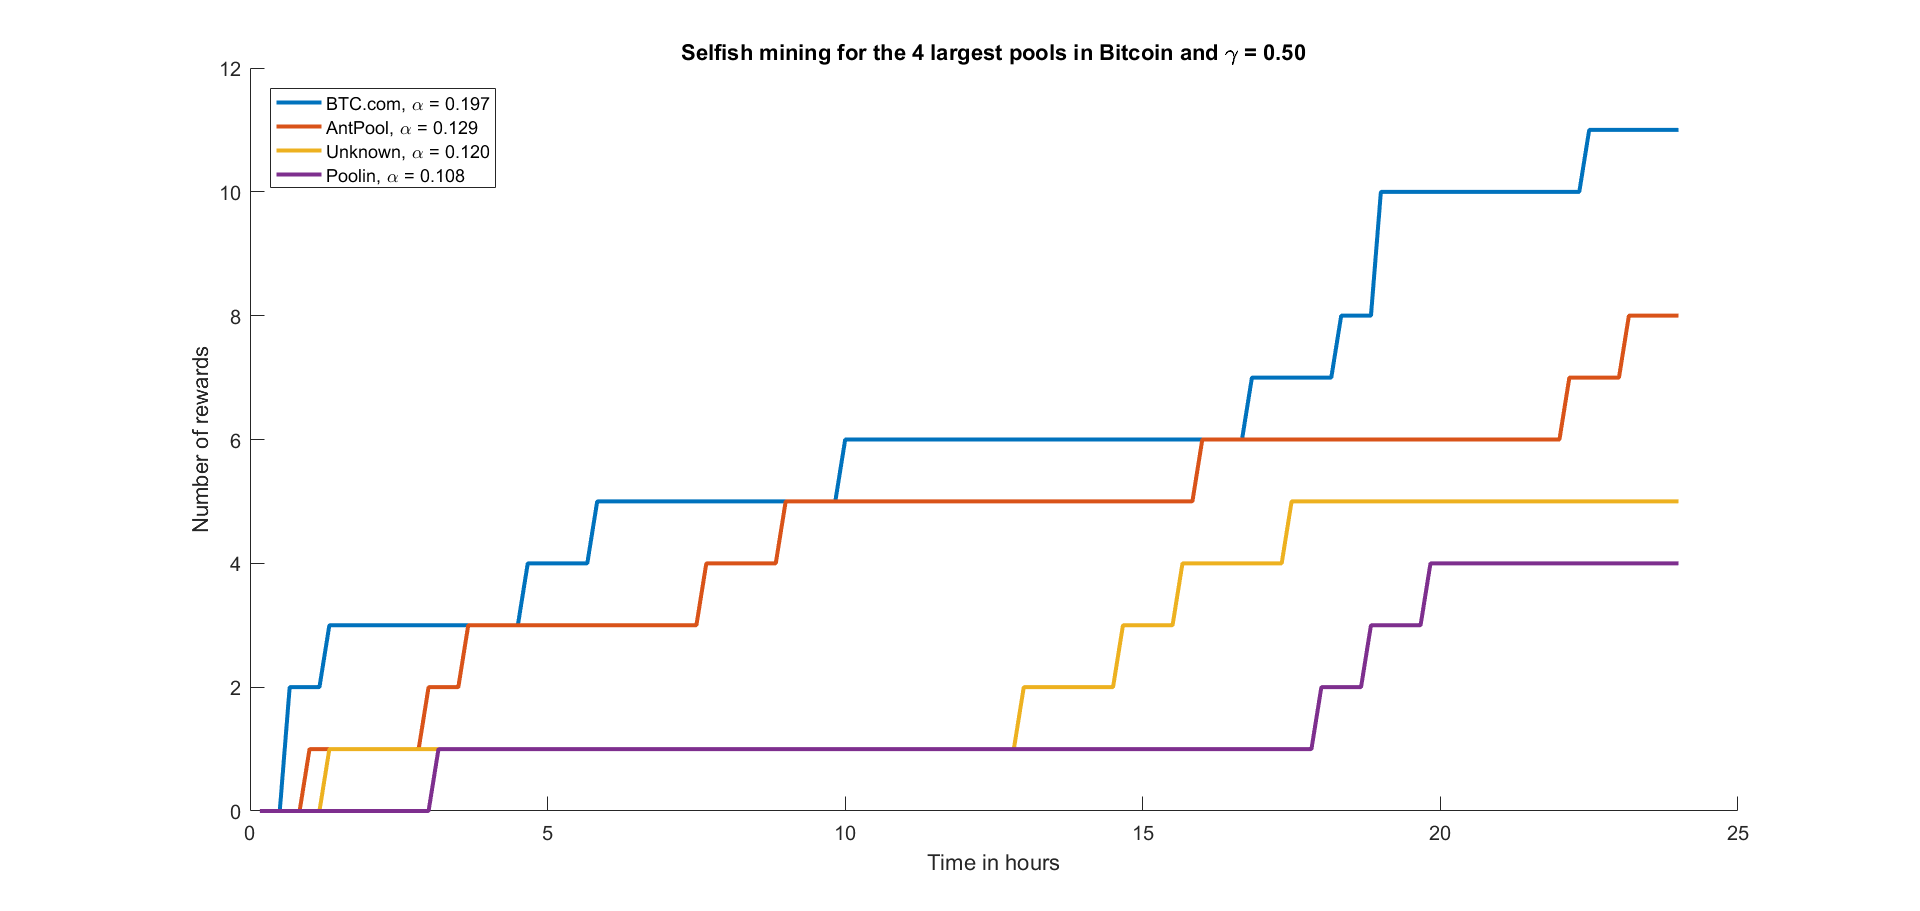
\includegraphics[width=12cm]{Figures/largestPools12}
} \newline
\end{figure}

\begin{figure}[ht]
\centering
\subfloat{
  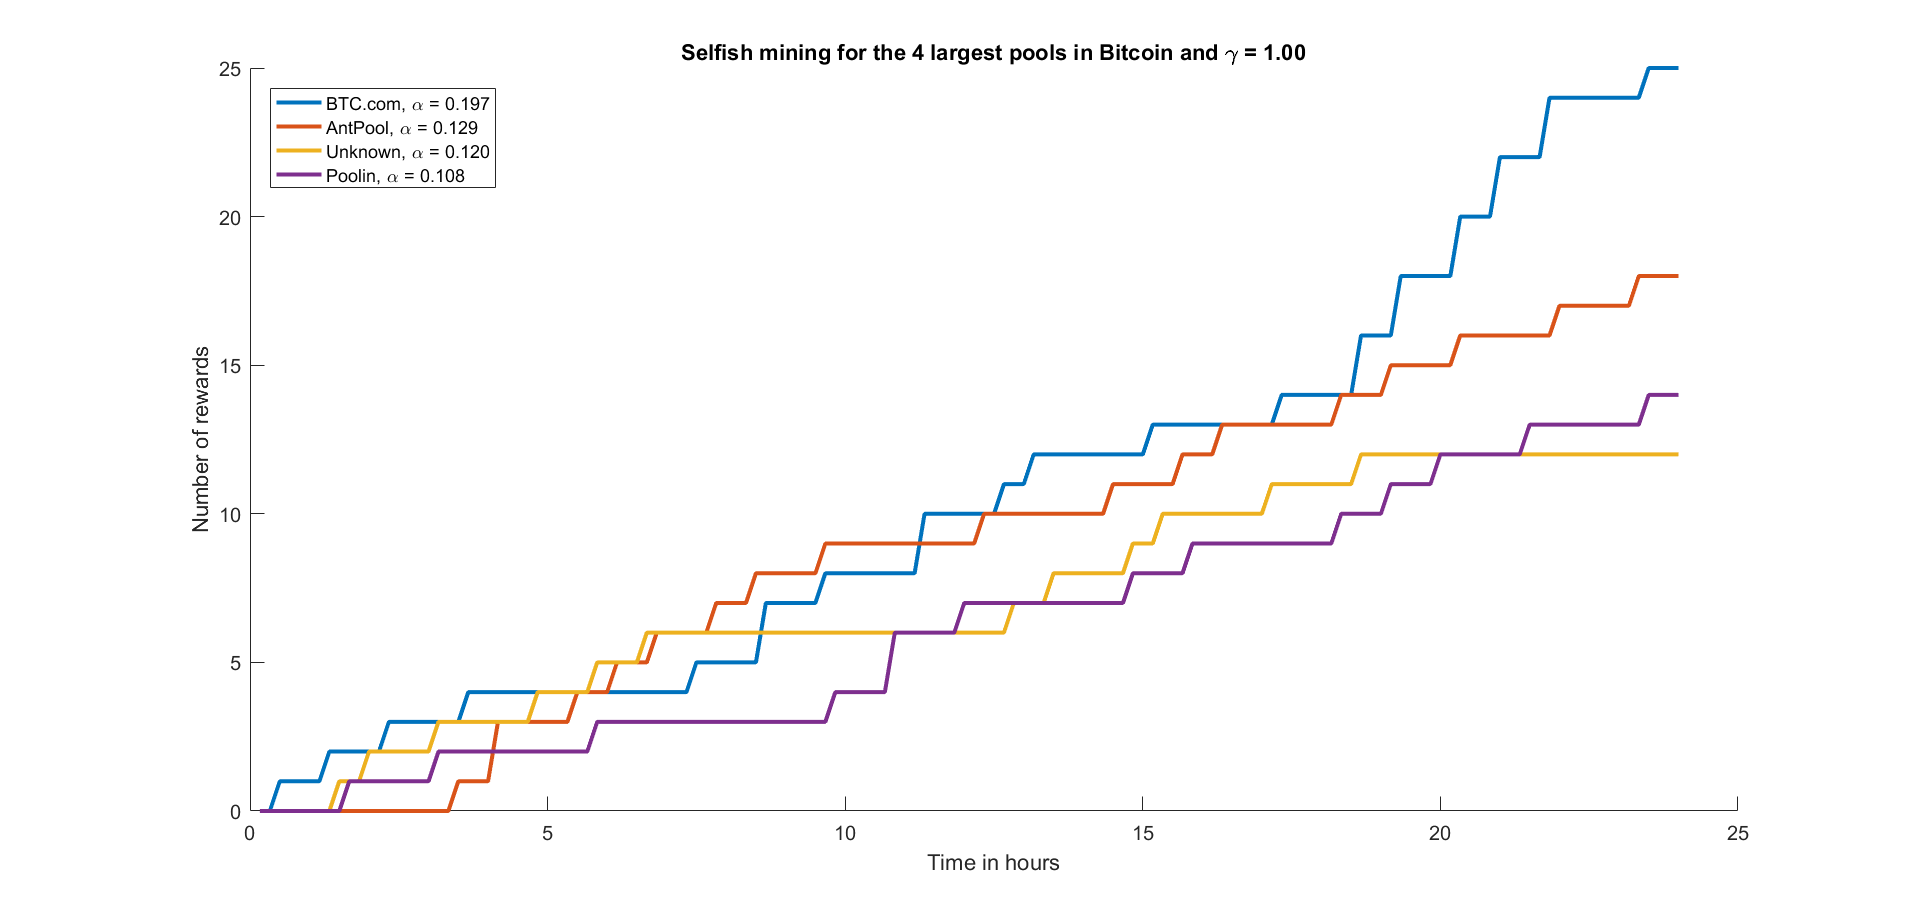
\includegraphics[width=12cm]{Figures/largestPools1}
} \newline
\end{figure}
\medskip

\clearpage
We can see that the pools will be able to win more if they can propagate their blocks fast enough, i.e. if $\gamma$ is high enough.

Now, we need to know if it's worth the effort against the honest mining, to do so we can analyze the link between $\alpha$ and $\gamma$ in the formulas for the revenues (Table \ref{revenueFormulas}) as it was done in \cite{majority_not_enough}. \newline

\begin{figure}[ht]
\centering
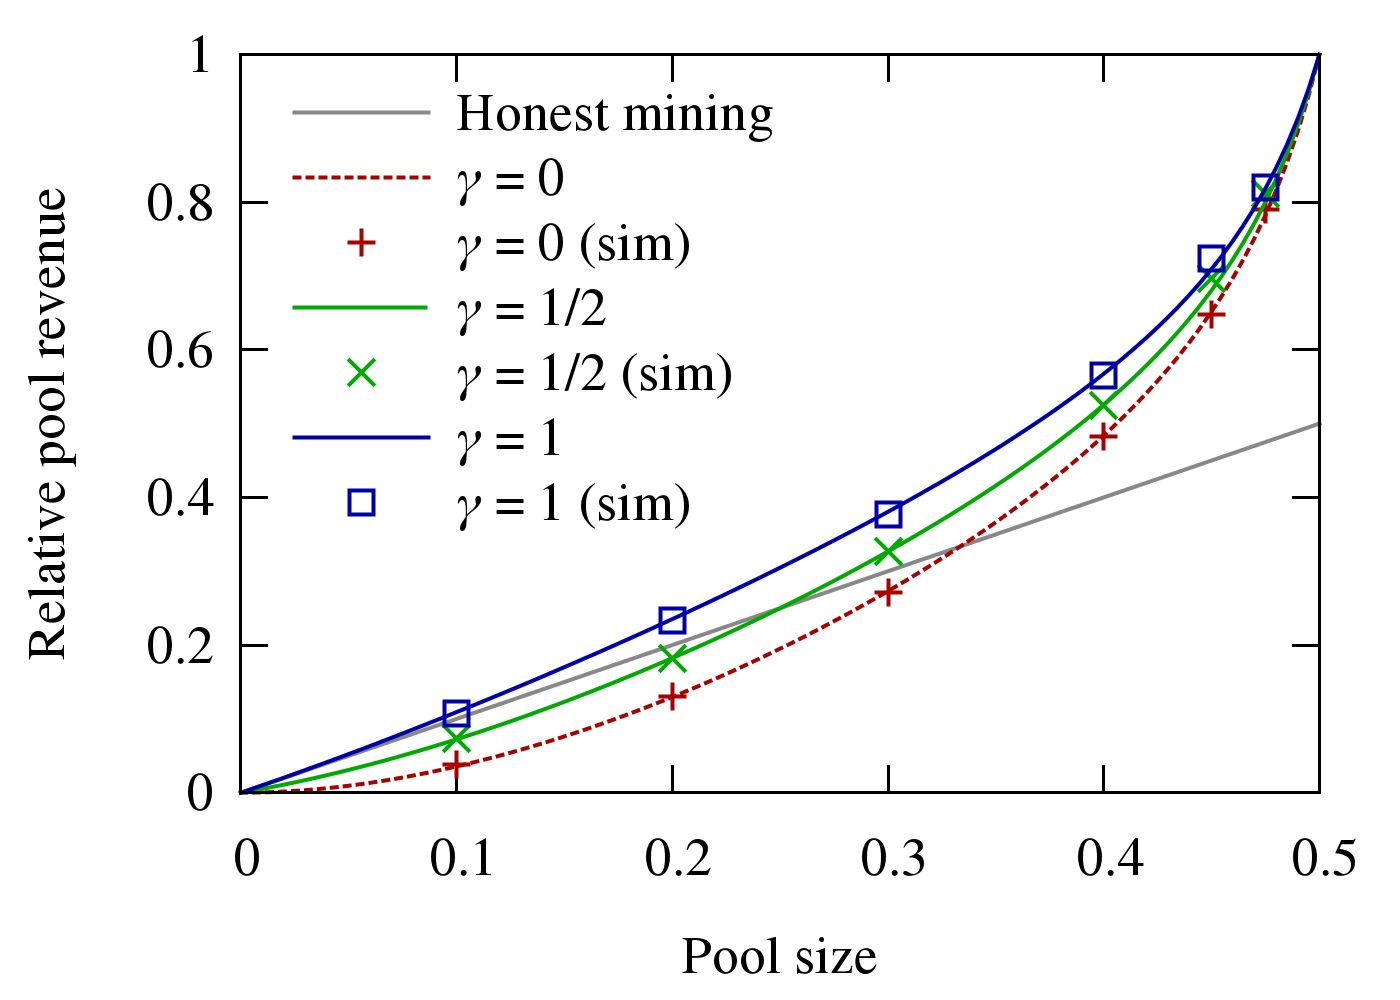
\includegraphics[width=10cm]{Figures/poolRevenue}
\caption{Revenue of the selfish miners for different values of $\alpha$ and $\gamma$}
\end{figure}
\medskip

This figure shows the importance of $\gamma$. With a high $\gamma$, the pool will propagate its blocks to the whole network very quickly so the selfish mining strategy will be efficient.

However, with a low $\gamma$, the honest miners will propagate their blocks quickly. If we take the extreme case of $\gamma = 0$, we'll need a pool with around 35\% of the mining power. For Bitcoin, the largest pool has 19.7\% of hash rate (see \cite{hashrate_pools}) so it seems secured for low $\gamma$.\newline

In Bitcoin, the protocol doesn't ensure that $\gamma$, which represents the propagation rate of the pools' miners, will stay low. This is because when an honest miner has several chains of the same length, he will choose to mine the first block he receives. Then, a pool can perform a Sybil attack, they use virtual miners who won't mine but when they detect that the honest miners have mined a new block, they propagate the pool's block so it will be broadcast faster and increase $\gamma$. \newline

A solution to this problem would be to change the protocol and make the miners to choose randomly between chains of the same length. This would lead to $\gamma = 1/2$ and it would require a pool with 25\% of hash rate, which is hard to achieve.


\chapter{Quantum computing and blockchains' security}

  Since the 1990s, quantum computing has become an important field of research in computer science. In 1998, we've seen the first quantum computer with 3 qubits and since then a lot of improvements and researches have been done to build a stable quantum computer. \newline

Let's anticipate the possible apogee of the quantum era and study how it could affect blockchains' security. We can watch some Youtube videos (see \cite{scienceEtonnante} and \cite{confTedEd}) as an introduction to quantum computers.

\section{What is Quantum computing?}

Quantum computing differs from classical computing by the way it stores and manipulates information. \newline

Let's have a quick reminder of how a classic computer works. \newline

They use bits to represent data, a bit can be either 0 or 1. Those two states are represented through an electrical signal. \newline

\begin{figure}[ht]
\centering
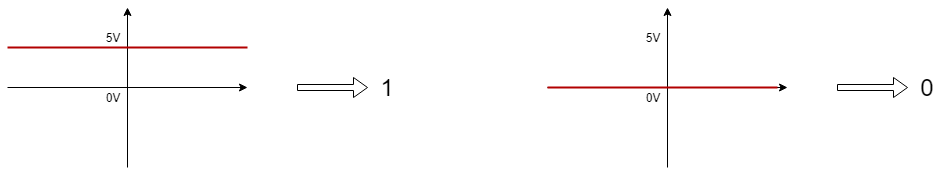
\includegraphics[width=14cm]{Figures/electricSignals}
\caption{Coding of a bit}
\end{figure}
\medskip

We process these signals with transistors to make logical gates, this is the basics of processors and computer architecture. To represent complex data, we create registers made of several bits. For example, a n-bits register can represent $2^n$ values/states. \newline

Now, what about quantum computing? (see \cite{qubitWiki}) As the name suggests, this new technology is based on quantum physics, the big difference with classic computers is that there aren't bits anymore but qubits or quantum bits. \newline

These qubits are not binary, either 0 or 1, but they exist in a superposition of 0 and 1. This is the superposition principle, we can understand it as probabilities so we commonly describe a qubit with the following formula: \newline

\begin{equation}
  \bra{x} = \alpha . \bra{0} + \beta . \bra{1}
\end{equation}
\medskip

where $\alpha$ is the probability for 0 and $\beta$ is the probability for 1. \newline

Mathematically, we can interpret these different states as coexisting but physically they're not, this is because quantum physic is not deterministic but probabilistic so we can't measure it precisely. \newline

It's important to highlight that a quantum computer isn't an evolution of classic computers like clusters can be. A whole new technology is involved in heading to a new way of representing and manipulating data. \newline

We won't go too far in the details about quantum physics and qubits but we can investigate two interesting questions. \newline

\paragraph{How do we physically build a qubit?}

There are different possibilities to build a qubit, we need to use a two-level system, a system where a quantum superposition can exist. For example, we could use photons and light polarization, where we measure how much the light is vertically or horizontally polarized. \newline

One famous method is to use the spins of the electrons (see \cite{spinWiki}) where we measure the spin angular momentum to describe the quantum state of the electron. This spin can be affected by the magnetic field around the particle. \newline

\begin{figure}[ht]
\centering
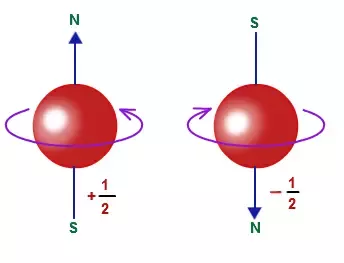
\includegraphics[width=6cm]{Figures/electronSpin}
\caption{Electron spin from \cite{spinNumber}}
\end{figure}
\medskip

These methods are more complicated than electric signals for classic bits, it's harder to keep the quantum bits stable. Researches are working on the stability of qubits to build bigger computers.

\paragraph{How can we recover the state form a qubit?}

Quantum computers follow a rule called "Wave function collapse", which says that a superposed state can't be known entirely, we can only measure it and so reduce it to one value.

This means that even if we have a $2^n$ superposed state, we will reduce it to one result. Then a quantum computer can be used only for specific problems with specifically designed algorithms like Grover algorithm. \newline

To conclude, a quantum computer will always be less polyvalent than its classical equivalent but it can be so much powerful for some specific problems. For example, it can be used for prime factorization, Peter Shor a scientist from Bell's lab found a quantum that could solve this problem. \newline


  \section{Is quantum computing a treat to blockchains' security ?}


  \section{How much are we close to build a quantum computer ?}

We've just seen that quantum computing can be a serious treat to blockchains' security and to cryptography in general. Now, we can wonder where are we in building a quantum computer ? \newline

As we already mentionned, quantum computers come up with a physical challenge because qubit aren't stable (see \cite{closeToQuantum}). Actually, there are different ways to implement a qubit but they are very sensitive to noise like temperature change or electrical fluctuation. A solution is to keep the circuits very cold, around the absolute zero (-273 degrees Celsius) but it involves large infrastructures.

So for now, there is still a need in research to put together large numbers of qubits (from a thousand to millions) but to keep it a reasonable size. \newline

Then, when can we hope to see the first 'real' quantum computers ? According to the recent improvements we made, we may think we're closed to the apogee, but in fact history has shown us that researches and advances take time. \newline

Some had even predicted quantum computers before 2019 but with the work left to do, 10 years seems to be a reasonable estimation.

\section{Do we have a contingency plan ?}

Let's have a look to the future and put ourselves in the quantum apogee. Actually, in parallel of the researches to develop quantum computing, some have found new algorithms and techniques to strengthen cryptography against quantum computers.

This new field of research is called post-quantum cryptography and some algorithms could be used to secure blockchains. In the actual version of the blockchain, we'll faced two issues against a quantum computer: \newline

\begin{itemize}
  \item Signature breakage: because RSA algorithm used for signing transactions will be broken. A easy solution is to change the public / private key of the sender at each transaction, this is already a recommended practice.
  \item As we mentioned, mining will be in danger. A solution will be to change the proof of work to be quantum resistant (see \cite{quantum_attacks}). Here are the basic properties we want for a proof of work: \newline

  \begin{enumerate}
    \item A adjustable difficulty according to the network computational power.
    \item The PoW is difficult to find but easy to verify.
    \item No advantage for quantum computers to find the PoW faster than a classical computer.
  \end{enumerate}
  \medskip

  The points 1 et 2 are already accomplished by the actual PoW. To satisfy point 3, an alternative is to base the difficulty to find the PoW not on computational power but on memory. \newline

  For example, we could use Momentum, a memory intensive proof of work based on finding birthday collisions (see \cite{momentum}). 
\end{itemize}


\appendix
\chapter{Complements about the target} \label{appendixTarget}

What does it imply to consider that the hash starts with d zeros? \newline

To simplify the analysis, we can assume that the condition of having a hash lower than the target is equivalent to start by d zeros, where d is 256 - exponent\_length. \newline

The "real" condition is harder to fulfill so how much work does it require if we only fulfill the second condition?
Let's suppose we find a hash starting with d zeros: \newline

$0 ... 0 a_1 a_2 a_3 a_4 a_5 a_6 0 ... 0$ \newline

and we have the following target: \newline

$0 ... 0 c_1 c_2 c_3 c_4 c_5 c_6 0 ... 0$ \newline

There are 3 possibilities: \newline

\begin{itemize}
  \item $a_1 < c_1$ : then the condition is fulfilled.
  \item $a_1 = c_1$ : we look at the next the bit and we are in the same situation for $c_2$, same for $c_3$, ..., $c_5$.
  \item $a_1 > c_1$ : we need a more bit of effort to satisfy the condition.
\end{itemize}

For $a_6$, if $a_6 = c_6$, we also need one more bit of effort to satisfy the condition.

Finally, whatever the situation, we need only one more bit of effort.

\chapter{Explanations on the revenues} \label{appendixRevenue}

In the chapter about selfish mining, we've calculated the revenues of the honest and selfish miners. \newline

\begin{table}[h]
  \centering

  \begin{tabular}{c}
    $r\_honest =  p_0 . (1 - \alpha) . 1 + p_{0'} . \gamma . (1 - \alpha) . 1 + p_{0'} . (1 - \gamma) (1 - \alpha) . 2$ \\
    \\
    $r\_selfish =  p_{0'} . \gamma . (1 - \alpha) . 1 + p_{0'} . \alpha . 2 + p_2 . (1 - \alpha) . 2 + P[i > 2] . (1 - \alpha) . 1$
  \end{tabular}
  \caption{Revenue won by the honest and selfish miners according to $\alpha$ and $\gamma$}
\end{table}
\medskip

Here is more explanations about these formulas : \newline

\begin{table}[h]

  \centering

  \begin{tabular}{l|l}
    $p_0 . (1 - \alpha) . 1$ & The honest miners find a block on the actual chain, they win 1 reward.\\
    \\
    $p_{0'} . \gamma . (1 - \alpha) . 1$ & \makecell[l]{The selfish and honest miners broadcast a block at the same time, then the honest miners \\ find the next block after the selfish miners' one, the honest and selfish miners win both 1 reward.}\\
    \\
    $p_{0'} . (1 - \gamma) (1 - \alpha) . 2$ & \makecell[l]{The selfish and honest miners broadcast a block at the same time, then the honest miners \\ find the next block after their own one, so they win 2 rewards.}\\
  \end{tabular}

  \vspace{1cm}

  \begin{tabular}{l|l}
    $p_{0'} . \gamma . (1 - \alpha) . 1$ & \makecell[l]{The selfish and honest miners broadcast a block at the same time, then the honest miners \\ find the next block after the selfish miners' one, the honest and selfish miners win both 1 reward.}\\
    \\
    $p_{0'} . \alpha . 2$ & \makecell[l]{The selfish and honest miners have both found a block, but the selfish miners find their \\ next block first, they publish both blocks and they win 2 rewards.}\\
    \\
    $p_2 . (1 - \alpha) . 2$ & \makecell[l]{The selfish miners had a lead of two blocks but the honest miners find one, so the selfish \\ miners publish their two blocks and they win 2 rewards.}\\
    \\
    $P[i > 2] . (1 - \alpha) . 1$ & Each time the selfish miners increase their lead above 2 blocks, they win 1 reward.\\
  \end{tabular}


  \caption{Explanations for the revenue of honest miners and selfish miners}

\end{table}


\nocite{*}
\bibliographystyle{IEEEtran}
\bibliography{IEEEabrv,biblio}
\addcontentsline{toc}{chapter}{Bibliography}

\end{document}
